% !TEX program = lualatex
% =====================================================================
%  Manual de usuario — Administrador del panel de cotizaciones
%  Training Corporation
%
%  Compilar (dos veces, para portada, índice y referencias):
%      lualatex manual-administrador.tex
%      lualatex manual-administrador.tex
%
%  Capturas de pantalla:
%      Guarde cada imagen en la carpeta capturas/ con el nombre que indica
%      su espacio en el PDF (por ejemplo capturas/02-01-login.png).
%      Se aceptan .png y .jpg. Al compilar de nuevo, la imagen reemplaza
%      el espacio automáticamente, ya enmarcada en la ventana del navegador.
% =====================================================================
\documentclass[11pt, a4paper, oneside]{report}

% ---------- Datos editables del documento ----------
\newcommand{\versiondoc}{1.0}
\newcommand{\fechadoc}{Noviembre de 2026}
\newcommand{\elaboradopor}{Equipo de desarrollo de Trainova}
% Dirección final de la aplicación: aparece en la barra del navegador de las capturas
% y en todas las direcciones del manual.
\newcommand{\dominio}{cotizaciones.\allowbreak trainingcorporation.\allowbreak com.\allowbreak co}

% =====================================================================
%  estilo.tex — Identidad visual del manual (Training Corporation)
%  Colores, tipografías, cajas, botones, capturas y diagramas.
%  Se carga desde manual-administrador.tex. Compilar con LuaLaTeX.
% =====================================================================

% ---------------------------------------------------------------------
%  Página
% ---------------------------------------------------------------------
\usepackage[a4paper, top=3cm, bottom=2.7cm, left=2.5cm, right=2.5cm,
            headheight=1.1cm, headsep=0.7cm, footskip=1.3cm]{geometry}

% ---------------------------------------------------------------------
%  Idioma y tipografías (las de la app: Montserrat + Source Sans 3)
% ---------------------------------------------------------------------
\usepackage{fontspec}
\usepackage{babel}
\babelprovide[import, main]{spanish}
\setlocalecaption{spanish}{contents}{Contenido}
\setlocalecaption{spanish}{listfigure}{Índice de figuras}
\setlocalecaption{spanish}{figure}{Figura}
\setlocalecaption{spanish}{table}{Tabla}
\setlocalecaption{spanish}{chapter}{Capítulo}
\setlocalecaption{spanish}{appendix}{Apéndice}

\setmainfont{SourceSans3}[
  Path           = fuentes/,
  Extension      = .otf,
  UprightFont    = *-Regular,
  ItalicFont     = *-It,
  BoldFont       = *-Bold,
  BoldItalicFont = *-BoldIt,
  FontFace       = {sb}{n}{*-Semibold},
  FontFace       = {sb}{it}{*-SemiboldIt},
]
\newfontfamily\montserrat{Montserrat}[
  Path        = fuentes/,
  Extension   = .otf,
  UprightFont = *-Regular,
  ItalicFont  = *-Italic,
  BoldFont    = *-Bold,
  FontFace    = {sb}{n}{*-SemiBold},
  FontFace    = {eb}{n}{*-ExtraBold},
  FontFace    = {ub}{n}{*-Black},
]
\newfontfamily\iconos{fa-solid-900}[Path = fuentes/, Extension = .ttf,
  BoldFont = *, ItalicFont = *, BoldItalicFont = *,
  FontFace = {sb}{n}{*}, FontFace = {eb}{n}{*}, FontFace = {ub}{n}{*},
  FontFace = {sb}{it}{*}, FontFace = {m}{it}{*}]

\linespread{1.1}
\setlength{\parindent}{0pt}
\setlength{\parskip}{0.55em plus 0.15em}
\setlength{\emergencystretch}{2.5em}

% ---------------------------------------------------------------------
%  Paquetes
% ---------------------------------------------------------------------
\usepackage{xcolor}
\usepackage{graphicx}
\usepackage{float}
\usepackage{tabularx}
\usepackage{tabularray}
\usepackage{enumitem}
\usepackage{titlesec}
\usepackage{titletoc}
\usepackage{fancyhdr}
\usepackage{caption}
\usepackage[most]{tcolorbox}
\usepackage{tikz}
\usetikzlibrary{calc, positioning, arrows.meta, shapes.symbols, shapes.misc,
                decorations.pathreplacing, fit, backgrounds}
\usepackage{microtype}

% ---------------------------------------------------------------------
%  Paleta (tailwind.config.js de la app)
% ---------------------------------------------------------------------
\definecolor{azul}{HTML}{0072AF}       % azul del logo
\definecolor{azulhondo}{HTML}{005A8C}  % hover / enlaces
\definecolor{azulvivo}{HTML}{1391DA}   % anillos y trazos
\definecolor{cielo}{HTML}{7FD0F5}      % acentos sobre noche
\definecolor{noche}{HTML}{0B2C47}      % azul marino de marca
\definecolor{tinta}{HTML}{102A3F}      % texto
\definecolor{pizarra}{HTML}{4A5A67}    % texto secundario
\definecolor{grismarca}{HTML}{8F9392}  % gris del logo
\definecolor{niebla}{HTML}{A9C6DC}     % texto secundario sobre noche
\definecolor{nube}{HTML}{EEF4F8}       % fondo alterno
\definecolor{linea}{HTML}{D5E2EB}      % bordes y reglas
\definecolor{error}{HTML}{B3261E}
% Insignias de estado (status-badge.tsx)
\definecolor{ambarfondo}{HTML}{FFFBEB}
\definecolor{ambarborde}{HTML}{FDE68A}
\definecolor{ambartexto}{HTML}{78350F}
\definecolor{verdefondo}{HTML}{ECFDF5}
\definecolor{verdeborde}{HTML}{A7F3D0}
\definecolor{verdetexto}{HTML}{065F46}
\definecolor{verde}{HTML}{1E7B4E}
\definecolor{errorfondo}{HTML}{FBEDEC}

\AtBeginDocument{\color{tinta}}

% ---------------------------------------------------------------------
%  Íconos (Font Awesome 6 Free, equivalentes a los de la app)
% ---------------------------------------------------------------------
\newcommand{\ico}[1]{{\iconos\char"#1\relax}}
\newcommand{\icVer}{\ico{F06E}}
\newcommand{\icEditar}{\ico{F303}}
\newcommand{\icEliminar}{\ico{F2ED}}
\newcommand{\icMas}{\ico{2B}}
\newcommand{\icBuscar}{\ico{F002}}
\newcommand{\icCerrar}{\ico{F00D}}
\newcommand{\icSubir}{\ico{F062}}
\newcommand{\icBajar}{\ico{F063}}
\newcommand{\icAtras}{\ico{F060}}
\newcommand{\icAnterior}{\ico{F053}}
\newcommand{\icSiguiente}{\ico{F054}}
\newcommand{\icSalir}{\ico{F2F5}}
\newcommand{\icExterno}{\ico{F08E}}
\newcommand{\icExcel}{\ico{F1C3}}
\newcommand{\icCargar}{\ico{F093}}
\newcommand{\icDescargar}{\ico{F019}}
\newcommand{\icPlay}{\ico{F04B}}
\newcommand{\icCopiar}{\ico{F0C5}}
\newcommand{\icCorreo}{\ico{F0E0}}
\newcommand{\icEnviar}{\ico{F1D8}}
\newcommand{\icAjustes}{\ico{F013}}
\newcommand{\icUsuarios}{\ico{F0C0}}
\newcommand{\icMaletin}{\ico{F0B1}}
\newcommand{\icRama}{\ico{F126}}
\newcommand{\icLlave}{\ico{F0AD}}
\newcommand{\icArbol}{\ico{F0E8}}
\newcommand{\icCotizacion}{\ico{F70E}}
\newcommand{\icContactos}{\ico{F2B9}}
\newcommand{\icMenu}{\ico{F0C9}}
\newcommand{\icOk}{\ico{F058}}
\newcommand{\icCandado}{\ico{F023}}
\newcommand{\icCasa}{\ico{F015}}
\newcommand{\icGlobo}{\ico{F0AC}}
\newcommand{\icClave}{\ico{F084}}
\newcommand{\icFlechaRama}{\ico{F149}}
\newcommand{\icMovil}{\ico{F3CD}}
\newcommand{\icDuplicar}{\ico{F24D}}

% ---------------------------------------------------------------------
%  Elementos de interfaz en el texto
% ---------------------------------------------------------------------
% Botón principal (azul), secundario (borde) y de peligro (rojo)
\newtcbox{\boton}{on line, colback=azul, colframe=azul, coltext=white,
  boxrule=0.6pt, arc=2.5pt, boxsep=0pt, left=4.5pt, right=4.5pt, top=1.8pt, bottom=1.8pt,
  fontupper=\montserrat\bfseries\fontsize{8.4}{10}\selectfont}
\newtcbox{\botonsec}{on line, colback=white, colframe=azul, coltext=azul,
  boxrule=0.8pt, arc=2.5pt, boxsep=0pt, left=4.5pt, right=4.5pt, top=1.6pt, bottom=1.6pt,
  fontupper=\montserrat\bfseries\fontsize{8.4}{10}\selectfont}
\newtcbox{\botonrojo}{on line, colback=white, colframe=error, coltext=error,
  boxrule=0.8pt, arc=2.5pt, boxsep=0pt, left=4.5pt, right=4.5pt, top=1.6pt, bottom=1.6pt,
  fontupper=\montserrat\bfseries\fontsize{8.4}{10}\selectfont}
% Nombre de un campo, columna o etiqueta de pantalla
\newtcbox{\campo}{on line, colback=nube, colframe=linea, coltext=noche,
  boxrule=0.5pt, arc=2pt, boxsep=0pt, left=3.5pt, right=3.5pt, top=1.2pt, bottom=1.2pt,
  fontupper=\fontseries{sb}\selectfont\small}
% Tecla del teclado
\newtcbox{\tecla}{on line, enhanced, colback=white, colframe=grismarca, coltext=noche,
  boxrule=0.6pt, bottomrule=1.6pt, arc=2pt, boxsep=0pt, left=3.5pt, right=3.5pt, top=1pt, bottom=1pt,
  fontupper=\montserrat\fontseries{sb}\selectfont\footnotesize}
% Insignias de estado
\newtcbox{\insignia}[1][]{on line, arc=6pt, boxsep=0pt, left=5pt, right=5pt,
  top=1pt, bottom=1.3pt, boxrule=0.6pt, fontupper=\fontseries{sb}\selectfont\footnotesize, #1}
\newcommand{\pendiente}{\insignia[colback=ambarfondo, colframe=ambarborde, coltext=ambartexto]{Pendiente}}
\newcommand{\generada}{\insignia[colback=verdefondo, colframe=verdeborde, coltext=verdetexto]{Generada}}
\newcommand{\vista}{\insignia[colback=nube, colframe=linea, coltext=azulhondo]{Vista}}
\newcommand{\novista}{\insignia[colback=nube, colframe=linea, coltext=tinta]{No vista}}
\newcommand{\insigniainfo}[1]{\insignia[colback=nube, colframe=linea, coltext=azulhondo]{#1}}
\newcommand{\insignianeutra}[1]{\insignia[colback=nube, colframe=linea, coltext=tinta]{#1}}

% Ruta de la barra lateral: grupo › opción
\newcommand{\menu}[2]{{\fontseries{sb}\selectfont\color{azulhondo}#1\hspace{0.35em}%
  {\iconos\fontsize{6.5}{8}\selectfont\raisebox{0.12em}{\char"F054}}\hspace{0.35em}#2}}
% Dirección (URL) de una pantalla
\newcommand{\ruta}[1]{{\ttfamily\small\color{azulhondo}#1}}
% Mensaje del sistema, copiado textualmente
\newcommand{\msg}[1]{«\textit{#1}»}
% Parte variable de un mensaje
\newcommand{\var}[1]{{\upshape\color{azulvivo}‹#1›}}
% Ícono de la app dentro del texto
\newcommand{\icono}[2][azul]{{\color{#1}#2}}

% Referencias cruzadas en color de enlace
\newcommand{\seccion}[1]{\hyperref[#1]{\textcolor{azulhondo}{\fontseries{sb}\selectfont sección~\ref*{#1}}}}
\newcommand{\capref}[1]{\hyperref[#1]{\textcolor{azulhondo}{\fontseries{sb}\selectfont capítulo~\ref*{#1}}}}
\newcommand{\apref}[1]{\hyperref[#1]{\textcolor{azulhondo}{\fontseries{sb}\selectfont apéndice~\ref*{#1}}}}
\newcommand{\Capref}[1]{\hyperref[#1]{\textcolor{azulhondo}{\fontseries{sb}\selectfont Capítulo~\ref*{#1}}}}
\newcommand{\Apref}[1]{\hyperref[#1]{\textcolor{azulhondo}{\fontseries{sb}\selectfont Apéndice~\ref*{#1}}}}
\newcommand{\figref}[1]{\hyperref[#1]{\textcolor{azulhondo}{\fontseries{sb}\selectfont figura~\ref*{#1}}}}
\newcommand{\pag}[1]{\hyperref[#1]{\textcolor{azulhondo}{pág.~\pageref*{#1}}}}

% Párrafo de entrada de cada capítulo
\newcommand{\entradilla}[1]{%
  {\fontsize{13}{19.5}\selectfont\color{pizarra}#1\par}\vspace{0.9em}}

% ---------------------------------------------------------------------
%  Listas: pasos numerados con el círculo azul de las tarjetas de la app
% ---------------------------------------------------------------------
\NewDocumentCommand{\circulopaso}{m}{\tikz[baseline=(n.base)]\node[circle, fill=azul, text=white,
  inner sep=0pt, minimum size=1.45em, font=\montserrat\bfseries\footnotesize] (n) {#1};}
\NewDocumentCommand{\circulozona}{m}{\tikz[baseline=(n.base)]\node[circle, fill=noche, text=white,
  inner sep=0pt, minimum size=1.45em, font=\montserrat\bfseries\footnotesize] (n) {#1};}

\newlist{pasos}{enumerate}{1}
\setlist[pasos]{label=\circulopaso{\arabic*}, leftmargin=2.3em, labelsep=0.65em,
  itemsep=0.45em, topsep=0.5em, parsep=0.25em}
\newlist{zonas}{enumerate}{1}
\setlist[zonas]{label=\circulozona{\Alph*}, leftmargin=2.3em, labelsep=0.65em,
  itemsep=0.35em, topsep=0.3em, parsep=0.2em}
\setlist[itemize,1]{label=\raisebox{0.18em}{\color{azul}\rule{0.38em}{0.38em}},
  leftmargin=1.5em, itemsep=0.25em, topsep=0.4em}
\setlist[itemize,2]{label=\raisebox{0.2em}{\color{azulvivo}\rule{0.3em}{0.3em}},
  leftmargin=1.3em}

% ---------------------------------------------------------------------
%  Cajas de aviso
% ---------------------------------------------------------------------
\tcbset{
  aviso/.style n args={4}{%  color, fondo, ícono, título
    enhanced, breakable, colback=#2, colframe=#1, coltext=tinta,
    boxrule=0pt, leftrule=3.5pt, arc=0pt, outer arc=0pt,
    left=11pt, right=11pt, top=8pt, bottom=8pt, before skip=10pt, after skip=10pt,
    before upper={{\color{#1}\iconos\char"#3\relax}\hspace{0.55em}%
      {\montserrat\bfseries\color{#1}#4}\par\vspace{2pt}},
  },
}
\newtcolorbox{nota}[1][Nota]{aviso={azul}{nube}{F05A}{#1}}
\newtcolorbox{importante}[1][Importante]{aviso={error}{errorfondo}{F071}{#1}}
\newtcolorbox{consejo}[1][Consejo]{aviso={azulvivo}{cielo!14!white}{F0EB}{#1}}
\newtcolorbox{resultado}[1][Resultado]{aviso={verde}{verdefondo}{F058}{#1}}

% Ficha de acceso al inicio de cada módulo
\NewDocumentCommand{\ficha}{m m m m}{%
  \begin{tcolorbox}[enhanced, colback=nube, colframe=linea, boxrule=0.6pt, arc=6pt,
      left=10pt, right=12pt, top=9pt, bottom=9pt, sidebyside, sidebyside align=top seam,
      lefthand width=1.2cm, sidebyside gap=12pt, segmentation hidden,
      before skip=6pt, after skip=12pt]
    \tikz\node[fill=azul, text=white, minimum size=1.2cm, inner sep=0pt, rounded corners=3pt,
      font=\fontsize{17}{17}\selectfont]{\ico{#1}};
    \tcblower
    \small
    \begin{tabularx}{\linewidth}{@{}l@{\hspace{10pt}}X@{}}
      {\montserrat\bfseries\scriptsize\color{pizarra}UBICACIÓN} & #2\\[3pt]
      {\montserrat\bfseries\scriptsize\color{pizarra}DIRECCIÓN} & \ruta{\dominio\allowbreak#3}\\[3pt]
      {\montserrat\bfseries\scriptsize\color{pizarra}PERMITE} & #4
    \end{tabularx}
  \end{tcolorbox}}

% ---------------------------------------------------------------------
%  Tablas (cabecera azul y filas alternas, como el Excel de clientes)
% ---------------------------------------------------------------------
\NewTblrEnviron{tabla}
\SetTblrInner[tabla]{
  rowsep = 4.5pt, colsep = 7pt,
  hlines = {fg=linea, wd=0.5pt},
  cells = {font=\small},
  row{even} = {bg=nube},
  row{1} = {bg=azul, fg=white, font=\montserrat\bfseries\footnotesize},
}
\SetTblrInner[longtblr]{
  rowsep = 4.5pt, colsep = 7pt,
  hlines = {fg=linea, wd=0.5pt},
  cells = {font=\small},
  row{even} = {bg=nube},
  row{1} = {bg=azul, fg=white, font=\montserrat\bfseries\footnotesize},
  rowhead = 1,
}
\SetTblrTemplate{head}{empty}
\SetTblrTemplate{foot}{empty}
\SetTblrOuter[longtblr]{entry=none, label=none}

% ---------------------------------------------------------------------
%  Capturas de pantalla
%  Si existe capturas/<archivo>.png (o .jpg) se muestra dentro de una
%  ventana de navegador; si no, aparece un espacio con instrucciones.
% ---------------------------------------------------------------------
\newcommand{\puntosnavegador}{\tikz[baseline=-0.55ex]{%
  \fill[error!75!white] (0,0) circle (0.085cm);
  \fill[ambarborde!80!orange] (0.3,0) circle (0.085cm);
  \fill[verdeborde!60!verde] (0.6,0) circle (0.085cm);}}
\newcommand{\barraurl}[1]{\tikz[baseline=(u.base)]\node[draw=linea, fill=white,
  rounded corners=6pt, text width=\dimexpr\linewidth-1.6cm\relax, align=left,
  inner xsep=7pt, inner ysep=2.3pt, font=\scriptsize, text=pizarra] (u)
  {{\iconos\fontsize{5.5}{6}\selectfont\char"F023}\hspace{0.5em}\dominio#1};}

\tcbset{
  navegador/.style={
    enhanced, colback=white, colframe=linea, boxrule=0.9pt, arc=5pt, sharp corners=south,
    colbacktitle=nube, coltitle=pizarra, titlerule=0.9pt, boxsep=0pt,
    left=0pt, right=0pt, top=0pt, bottom=0pt, halign=center,
    toptitle=4pt, bottomtitle=4pt, lefttitle=8pt, righttitle=8pt,
    fonttitle=\scriptsize, title={\puntosnavegador\hspace{0.7em}\barraurl{#1}},
  },
  telefono/.style={
    enhanced, center, width=6.4cm, colback=white, colframe=noche, boxrule=5pt, arc=16pt,
    boxsep=0pt, left=0pt, right=0pt, top=13pt, bottom=9pt, halign=center,
    overlay={\fill[grismarca!70, rounded corners=1pt]
      ([xshift=-0.65cm, yshift=-7pt]frame.north) rectangle ([xshift=0.65cm, yshift=-9.5pt]frame.north);},
  },
}

\newcommand{\espaciocaptura}[3]{% alto, archivo, qué capturar
  \begin{tikzpicture}
    \path[use as bounding box] (0,0) rectangle (\linewidth,#1);
    \fill[nube!70] (0,0) rectangle (\linewidth,#1);
    \draw[azulvivo!75, line width=0.9pt, dash pattern=on 5pt off 3pt, rounded corners=5pt]
      (8pt,8pt) rectangle (\linewidth-8pt,#1-8pt);
    \node[text width=0.8\linewidth, align=center, font=\small, text=pizarra]
      at (0.5\linewidth,0.5*#1) {%
        {\iconos\fontsize{24}{24}\selectfont\color{azulvivo}\char"F030}\\[6pt]
        {\montserrat\bfseries\color{azul}Espacio para la captura}\\[2pt]
        {\ttfamily\footnotesize\color{azulhondo}capturas/#2.png}\\[7pt]
        {\color{tinta}\textbf{Qué capturar:}}~#3};
  \end{tikzpicture}}

% Todas las capturas se dibujan con la misma escala de texto: una captura de escritorio de
% 892 px de ancho (CSS) llena el ancho del texto; las más angostas quedan proporcionalmente
% más pequeñas y las más anchas se ajustan al margen. Las imágenes son de doble densidad.
\newlength{\anchonatural}
\newcommand{\escalacaptura}{0.2543}
\newcommand{\incluircaptura}[1]{%
  \settowidth{\anchonatural}{\includegraphics{#1}}%
  \setlength{\anchonatural}{\escalacaptura\anchonatural}%
  \ifdim\anchonatural>\linewidth \setlength{\anchonatural}{\linewidth}\fi
  \includegraphics[width=\anchonatural, height=0.6\textheight, keepaspectratio]{#1}}

\newcommand{\imagencaptura}[3]{% archivo, alto del espacio, qué capturar
  \IfFileExists{capturas/#1.png}%
    {\incluircaptura{capturas/#1.png}}%
    {\IfFileExists{capturas/#1.jpg}%
      {\incluircaptura{capturas/#1.jpg}}%
      {\espaciocaptura{#2}{#1}{#3}}}}

% \captura[alto del espacio]{archivo}{ruta}{pie de figura}{qué capturar}
\NewDocumentCommand{\captura}{O{7cm} m m m m}{%
  \begin{figure}[H]
    \begin{tcolorbox}[navegador={#3}]
      \imagencaptura{#2}{#1}{#5}
    \end{tcolorbox}
    \caption{#4}\label{fig:#2}
  \end{figure}}

% \capturaventana[alto]{archivo}{título de la ventana}{pie}{qué capturar}
% Para capturas fuera del navegador (por ejemplo, un archivo de Excel).
\NewDocumentCommand{\capturaventana}{O{7cm} m m m m}{%
  \begin{figure}[H]
    \begin{tcolorbox}[navegador={}, title={\puntosnavegador\hspace{0.9em}%
        {\color{verde}\ico{F1C3}}\hspace{0.5em}{\fontseries{sb}\selectfont #3}}]
      \imagencaptura{#2}{#1}{#5}
    \end{tcolorbox}
    \caption{#4}\label{fig:#2}
  \end{figure}}


% \capturaconnotas[alto]{archivo}{ruta}{pie}{qué capturar}{texto a la derecha}
\NewDocumentCommand{\capturaconnotas}{O{10cm} m m m m +m}{%
  \begin{figure}[H]
    \begin{minipage}[t]{0.42\linewidth}\vspace{0pt}
      \begin{tcolorbox}[navegador={#3}]
        \imagencaptura{#2}{#1}{#5}
      \end{tcolorbox}
    \end{minipage}\hfill
    \begin{minipage}[t]{0.53\linewidth}\vspace{0pt}
      \small #6
    \end{minipage}
    \caption{#4}\label{fig:#2}
  \end{figure}}

% \capturamovil[alto]{archivo}{pie}{qué capturar}
\NewDocumentCommand{\capturamovil}{O{10.5cm} m m m}{%
  \begin{figure}[H]
        \begin{tcolorbox}[telefono]
      \renewcommand{\escalacaptura}{1}%
      \imagencaptura{#2}{#1}{#4}
    \end{tcolorbox}
    \caption{#3}\label{fig:#2}
  \end{figure}}

% ---------------------------------------------------------------------
%  Pies de figura
% ---------------------------------------------------------------------
\DeclareCaptionFont{pizarra}{\color{pizarra}}
\DeclareCaptionFont{azul}{\color{azul}}
\DeclareCaptionFont{montserrat}{\montserrat}
\DeclareCaptionLabelSeparator{punto}{.\enspace}
\captionsetup{font={small,pizarra}, labelfont={montserrat,bf,azul}, labelsep=punto,
  justification=centering, skip=7pt}
\captionsetup[figure]{position=below}

% ---------------------------------------------------------------------
%  El anillo abierto del logo (brand-ring.tsx), como dibujo TikZ
%  Uso: \pic at (x,y) {anillo={radio/grosor/color}};
% ---------------------------------------------------------------------
\tikzset{
  pics/anillo/.style args={#1/#2/#3}{
    code={
      \draw[#3, line width=#2, line cap=round] (25:#1) arc[start angle=25, end angle=335, radius=#1];
      \fill[#3] (90:#1) circle[radius=2.3*#2];
    }
  },
  tarjeta/.style={draw=linea, line width=0.9pt, fill=white, rounded corners=4pt,
    inner xsep=9pt, inner ysep=7pt, align=left},
  pastilla/.style n args={3}{rounded corners=5pt, draw=#1, fill=#2, text=#3,
    font=\fontseries{sb}\selectfont\scriptsize, inner xsep=5pt, inner ysep=1.6pt},
  flecha/.style={-{Stealth[length=6pt, width=5pt]}, azulvivo, line width=1.1pt},
}

% ---------------------------------------------------------------------
%  Títulos de capítulo: banda azul con número grande y anillos
% ---------------------------------------------------------------------
\newif\ifapendices
\newcommand{\etiquetanumero}{\ifapendices\thechapter\else\ifnum\value{chapter}<10 0\fi\arabic{chapter}\fi}
\newcommand{\etiquetacapitulo}{\ifapendices APÉNDICE\else CAPÍTULO\fi}

\newcommand{\anillosbanda}{%
  \begin{scope}
    \clip (current page.north west) rectangle ([yshift=-7cm]current page.north east);
    \pic[opacity=0.45] at ([xshift=-3.1cm, yshift=-2.7cm]current page.north east) {anillo={4.3cm/1.5pt/cielo}};
    \pic[opacity=0.7] at ([xshift=-0.5cm, yshift=-6.5cm]current page.north east) {anillo={1.9cm/1.1pt/azulvivo}};
  \end{scope}}

\newcommand{\bandacapitulo}[1]{%
  \begin{tikzpicture}[remember picture, overlay]
    \fill[azul] (current page.north west) rectangle ([yshift=-7cm]current page.north east);
    \anillosbanda
    \node[anchor=south west, inner sep=0pt, text=white,
      font=\montserrat\fontseries{ub}\selectfont\fontsize{68}{68}\selectfont] (num)
      at ([xshift=2.4cm, yshift=-5.85cm]current page.north west) {\etiquetanumero};
    \node[anchor=south west, inner sep=0pt, text=cielo,
      font=\montserrat\bfseries\fontsize{9.5}{11}\selectfont]
      at ([yshift=0.38cm]num.north west) {\addfontfeatures{LetterSpace=20}\etiquetacapitulo};
    \node[anchor=south west, inner sep=0pt, text width=10.6cm, align=left, text=white,
      font=\montserrat\fontseries{eb}\selectfont\fontsize{24}{28}\selectfont]
      at ([xshift=0.75cm, yshift=0.1cm]num.south east) {#1};
  \end{tikzpicture}%
  \par\vspace*{3.3cm}}

\newcommand{\bandacapitulosin}[1]{%
  \begin{tikzpicture}[remember picture, overlay]
    \fill[azul] (current page.north west) rectangle ([yshift=-7cm]current page.north east);
    \anillosbanda
    \node[anchor=south west, inner sep=0pt, text width=14cm, align=left, text=white,
      font=\montserrat\fontseries{eb}\selectfont\fontsize{30}{34}\selectfont]
      at ([xshift=2.4cm, yshift=-5.85cm]current page.north west) {#1};
  \end{tikzpicture}%
  \par\vspace*{3.3cm}}

\titleformat{\chapter}[block]{}{}{0pt}{\bandacapitulo}
\titleformat{name=\chapter, numberless}[block]{}{}{0pt}{\bandacapitulosin}
\titlespacing*{\chapter}{0pt}{0pt}{0pt}

\newcommand{\cajanumero}[1]{\tikz[baseline=(n.base)]\node[fill=azul, text=white, inner xsep=5pt,
  inner ysep=3.5pt, font=\montserrat\bfseries\fontsize{11}{11}\selectfont] (n) {#1};}
\titleformat{\section}{\montserrat\bfseries\fontsize{16}{20}\selectfont\color{azul}}
  {\cajanumero{\thesection}}{0.55em}{}
\titlespacing*{\section}{0pt}{1.9em plus 0.4em}{0.8em}
\titleformat{\subsection}{\montserrat\fontseries{sb}\selectfont\fontsize{12.5}{16}\selectfont\color{noche}}
  {\textcolor{azulvivo}{\thesubsection}}{0.6em}{}
\titlespacing*{\subsection}{0pt}{1.5em plus 0.3em}{0.5em}
\titleformat{\subsubsection}{\montserrat\bfseries\fontsize{10.5}{13}\selectfont\color{azulhondo}}
  {}{0pt}{}
\titlespacing*{\subsubsection}{0pt}{1.1em}{0.3em}
\setcounter{secnumdepth}{2}
\setcounter{tocdepth}{1}

% ---------------------------------------------------------------------
%  Índice
% ---------------------------------------------------------------------
\newcommand{\cajatoc}[1]{\tikz[baseline=(n.base)]\node[fill=azul, text=white, minimum width=1.9em,
  minimum height=1.5em, inner sep=0pt, font=\montserrat\bfseries\small] (n) {#1};}
\titlecontents{chapter}[3.1em]
  {\addvspace{10pt}\montserrat\bfseries\fontsize{11.5}{14}\selectfont\color{noche}}
  {\contentslabel[\cajatoc{\thecontentslabel}]{3.1em}}
  {\hspace*{-3.1em}}
  {\hfill\textcolor{azul}{\contentspage}}
\titlecontents{section}[5.7em]
  {\addvspace{1.5pt}\color{tinta}}
  {\contentslabel[\textcolor{azulvivo}{\montserrat\fontseries{sb}\selectfont\small\thecontentslabel}]{2.6em}}
  {\hspace*{-2.6em}}
  {\titlerule*[0.7pc]{\textcolor{linea}{.}}\contentspage}
\titlecontents{figure}[3.4em]
  {\addvspace{1pt}\small\color{tinta}}
  {\contentslabel[\textcolor{azul}{\montserrat\fontseries{sb}\selectfont\thecontentslabel}]{3.4em}}
  {}
  {\titlerule*[0.7pc]{\textcolor{linea}{.}}\contentspage}

% ---------------------------------------------------------------------
%  Encabezado y pie de página
% ---------------------------------------------------------------------
\newcommand{\numpagina}{\tikz[baseline=(p.base)]\node[fill=azul, text=white,
  font=\montserrat\bfseries\footnotesize, minimum width=0.85cm, minimum height=0.6cm,
  inner sep=2pt] (p) {\thepage};}
\newcommand{\textopie}{{\footnotesize\color{pizarra}Manual del administrador
  \textperiodcentered\ Trainova \textperiodcentered\ Versión \versiondoc}}

\pagestyle{fancy}
\fancyhf{}
\fancyhead[L]{\raisebox{-0.15cm}{
\includegraphics[height=0.75cm]{imagenes/logo.png}}}
\fancyhead[R]{{\montserrat\fontseries{sb}\selectfont\footnotesize\color{pizarra}\leftmark}}
\fancyfoot[L]{\textopie}
\fancyfoot[R]{\numpagina}
\renewcommand{\headrulewidth}{0.8pt}
\renewcommand{\headrule}{\hbox to\headwidth{\color{linea}\leaders\hrule height\headrulewidth\hfill}}
\renewcommand{\chaptermark}[1]{\markboth{\ifapendices Apéndice\else Capítulo\fi\ \thechapter
  \ \textperiodcentered\ #1}{}}
\fancypagestyle{plain}{%
  \fancyhf{}
  \fancyfoot[L]{\textopie}
  \fancyfoot[R]{\numpagina}
  \renewcommand{\headrulewidth}{0pt}
  \renewcommand{\headrule}{}}

% ---------------------------------------------------------------------
%  Portada
% ---------------------------------------------------------------------
\newcommand{\filaportada}[4]{% x, y, ícono, texto
  \node[fill=azul, text=white, minimum size=0.72cm, inner sep=0pt, rounded corners=2pt,
    font=\fontsize{10}{10}\selectfont] at (#1+0.36,#2) {\ico{#3}};
  \node[anchor=west, text width=6.4cm, align=left, inner sep=0pt, text=noche,
    font=\montserrat\fontseries{sb}\selectfont\fontsize{10.5}{13}\selectfont] at (#1+1.0,#2) {#4};}

\newcommand{\portada}{%
  \begin{titlepage}
  \thispagestyle{empty}
  \begin{tikzpicture}[remember picture, overlay, shift={(current page.south west)}]
    % Campo azul desde el borde superior, con los anillos de la marca como trama
    \fill[azul] (0,12.4) rectangle (21,29.7);
    \begin{scope}
      \clip (0,12.4) rectangle (21,29.7);
      \pic[opacity=0.30] at (19.6,14.2) {anillo={6.0cm/1.7pt/cielo}};
      \pic[opacity=0.65] at (20.6,27.0) {anillo={2.6cm/1.1pt/azulvivo}};
    \end{scope}
    % Título
    \node[anchor=north west, inner sep=0pt, text=cielo, font=\montserrat\bfseries\fontsize{10.5}{12}\selectfont]
      at (2.4,26.0) {\addfontfeatures{LetterSpace=18}MANUAL DE USUARIO};
    \node[anchor=north west, inner sep=0pt, text=white,
      font=\montserrat\fontseries{ub}\selectfont\fontsize{62}{66}\selectfont]
      at (2.4,25.3) {Trainova};
    \node[anchor=north west, inner sep=0pt, text width=16.2cm, align=left, text=white,
      font=\montserrat\fontseries{eb}\selectfont\fontsize{26}{31}\selectfont]
      at (2.4,22.75) {Administrador del\\panel de cotizaciones};
    \fill[cielo] (2.4,19.85) rectangle (4.9,19.97);
    \node[anchor=north west, inner sep=0pt, text width=13.8cm, align=left, text=white,
      font=\fontsize{13.5}{19}\selectfont] at (2.4,19.45)
      {Guía paso a paso, con capturas de pantalla, de todo lo que puede hacer el usuario
       administrador: desde el inicio de sesión hasta el cierre de sesión.};
    \node[anchor=north west, inner sep=0pt, text=cielo, font=\montserrat\fontseries{sb}\selectfont\fontsize{13}{16}\selectfont]
      at (2.4,16.6) {\dominio};
    % Contenido del manual, en dos columnas
    \node[anchor=west, inner sep=0pt, text=pizarra, font=\montserrat\bfseries\fontsize{8}{10}\selectfont]
      at (2.4,10.9) {\addfontfeatures{LetterSpace=18}EN ESTE MANUAL};
    \filaportada{2.4}{9.7}{F084}{Acceso al panel}
    \filaportada{2.4}{8.5}{F70E}{Cotizaciones y clientes}
    \filaportada{2.4}{7.3}{F0E8}{Catálogo y árbol de decisión}
    \filaportada{11.0}{9.7}{F013}{Usuarios, correos y configuración}
    \filaportada{11.0}{8.5}{F2F5}{Ver el sitio y cerrar sesión}
    \filaportada{11.0}{7.3}{F080}{Capacidad de la aplicación}
    % Franja inferior
    \fill[noche] (0,0) rectangle (21,2.7);
    \node[anchor=west, inner sep=0pt] at (2.4,1.35) {
\includegraphics[height=1.15cm]{imagenes/logo-blanco.png}};
    \node[anchor=east, align=right, inner sep=0pt, text=niebla, font=\small] at (18.6,1.35)
      {{\montserrat\bfseries\color{white}Versión \versiondoc}\\ \fechadoc};
  \end{tikzpicture}
  \end{titlepage}}

% ---------------------------------------------------------------------
%  Contraportada
% ---------------------------------------------------------------------
\newcommand{\contraportada}{%
  \clearpage
  \thispagestyle{empty}
  \begin{tikzpicture}[remember picture, overlay, shift={(current page.south west)}]
    \fill[noche] (0,0) rectangle (21,29.7);
    \begin{scope}
      \clip (0,0) rectangle (21,29.7);
      \pic[opacity=0.35] at (10.5,15.6) {anillo={6.2cm/1.6pt/cielo}};
      \pic[opacity=0.5] at (19.4,3.0) {anillo={3.2cm/1.1pt/azulvivo}};
      \pic[opacity=0.5] at (1.4,26.8) {anillo={2.4cm/1.1pt/azulvivo}};
    \end{scope}
    \node at (10.5,15.6) {
\includegraphics[width=6.4cm]{imagenes/logo-blanco.png}};
    \node[text=niebla, font=\small, align=center] at (10.5,5.2)
      {{\montserrat\bfseries\color{white}Training Corporation}\\[3pt]
              \dominio};
    \node[text=bruma, font=\footnotesize] at (10.5,3.9)
      {Trainova \textperiodcentered\ Manual del administrador \textperiodcentered\ Versión \versiondoc\ \textperiodcentered\ \fechadoc};
  \end{tikzpicture}
  \null}

\definecolor{bruma}{HTML}{93ABC0}

% ---------------------------------------------------------------------
%  Enlaces del PDF
% ---------------------------------------------------------------------
\usepackage[hidelinks, unicode, bookmarksnumbered]{hyperref}
\hypersetup{
  pdftitle   = {Trainova: manual de usuario del administrador},
  pdfauthor  = {Training Corporation},
  pdfsubject = {Guía paso a paso del panel de administración de Trainova},
  pdfkeywords= {Trainova, cotizaciones, manual, administrador, Training Corporation},
}
\usepackage{bookmark}


\begin{document}

\portada

\pagenumbering{roman}

\chapter*{Acerca de este manual}
\markboth{Acerca de este manual}{}

\entradilla{Este documento guía al usuario administrador en el uso diario del panel de
administración de Trainova, la plataforma de cotizaciones de Training Corporation. Cada tarea
se explica paso a paso y va acompañada de la captura de la pantalla correspondiente.}

\begin{tabla}{colspec={Q[4.2cm,l] X[l]}}
  Dato & Detalle \\
  Documento & Manual de usuario del administrador de Trainova \\
  Dirigido a & Personas con una cuenta de acceso al panel de administración de Trainova \\
  Aplicación & Trainova, plataforma de cotizaciones de Training Corporation (\ruta{\dominio}) \\
  Versión & \versiondoc \\
  Fecha & \fechadoc \\
  Elaborado por & \elaboradopor \\
\end{tabla}

\section*{Control de cambios}

\begin{tabla}{colspec={Q[2cm,c] Q[3.2cm,l] X[l]}}
  Versión & Fecha & Descripción \\
  1.0 & \fechadoc & Primera versión del manual: acceso, operación, catálogo, sistema, cierre de sesión y capacidad de la aplicación. \\
\end{tabla}

\begin{nota}[Sobre los textos de pantalla]
Los nombres de botones, campos y mensajes que aparecen en este manual se copiaron de la
aplicación tal como el usuario los ve. Si en una versión futura cambia algún texto en pantalla,
actualice también este documento.
\end{nota}

\tableofcontents
\listoffigures

\clearpage
\pagenumbering{arabic}

% =====================================================================
%  Capítulo 1 — Introducción
% =====================================================================
\chapter{Introducción}\label{cap:intro}

\entradilla{Antes de empezar, conozca qué es el panel de cotizaciones, qué puede hacer en él y
cómo está organizado este manual.}

\section{¿Qué es el panel de cotizaciones?}\label{sec:que-es}

\textbf{Training~InnovaQuote} es la plataforma web donde los clientes de Training Corporation solicitan
cotizaciones. Está disponible en \ruta{\dominio}. El cliente elige el tipo de servicio (la
\emph{unidad de negocio}), diligencia el \emph{formulario de solicitud} y envía su solicitud.

El \textbf{panel de cotizaciones} es la parte privada de Training~InnovaQuote. Desde allí el equipo de
Training Corporation recibe las solicitudes, envía las propuestas comerciales y mantiene al día
la información que ve el cliente. En el panel usted puede:

\begin{itemize}
  \item Revisar las solicitudes de cotización y enviar la propuesta a cada cliente.
  \item Consultar los clientes que han cotizado y su historial, y exportarlos a Excel.
  \item Administrar las unidades de negocio, las líneas de gestión y los servicios.
  \item Diseñar el formulario de preguntas (árbol de decisión) que responde el cliente al cotizar.
  \item Crear y administrar las cuentas de acceso al panel.
  \item Enviar correos de bienvenida para invitar clientes a la plataforma.
  \item Definir quién recibe las notificaciones y los datos de contacto que llevan los correos.
\end{itemize}

\section{El nombre Training InnovaQuote}\label{sec:nombre}

El nombre de la aplicación une tres palabras, y cada una expresa una parte de lo que es:

\begin{figure}[H]
\centering
\begin{tikzpicture}
  \node[font=\montserrat\fontseries{ub}\selectfont\fontsize{38}{38}\selectfont, inner sep=0pt] (n)
    {\textcolor{noche}{Training}\hspace{0.28em}\textcolor{azul}{Innova}\textcolor{azulvivo}{Quote}};
  \foreach \x/\col/\parte/\icono/\texto in {
      -5.1/noche/Training/F19C/{Respaldo e identidad de Training Corporation},
      0/azul/Innova/F0EB/{Innovación y transformación},
      5.1/azulvivo/Quote/F70E/{Cotizaciones y propuestas comerciales}} {
    \node[tarjeta, draw=\col!60, line width=1.2pt, text width=4.1cm, minimum height=2.9cm,
        align=center, inner ysep=9pt] at (\x,-2.75)
      {{\color{\col}\fontsize{15}{15}\selectfont\ico{\icono}}\\[5pt]
       {\montserrat\fontseries{eb}\selectfont\Large\color{\col}\parte}\\[4pt]
       {\small\color{tinta}\texto}};
  }
\end{tikzpicture}
\caption{Significado del nombre Training InnovaQuote.}\label{fig:nombre}
\end{figure}

\begin{tabla}{colspec={Q[3.2cm,l] X[l]}}
  Palabra & Significado \\
  \textbf{Training} & Respaldo e identidad de Training Corporation. \\
  \textbf{Innova} & Innovación y transformación. \\
  \textbf{Quote} & Cotizaciones y propuestas comerciales. \\
\end{tabla}

\section{¿Quién es el usuario administrador?}\label{sec:quien}

Toda persona que tenga una cuenta en el panel es administrador. El panel no maneja roles ni
permisos distintos: cualquier usuario puede ver y modificar todos los módulos, incluidas las
cuentas de los demás usuarios.

\begin{importante}
Entregue cuentas solo a personas de confianza y cree una cuenta por persona. No comparta su
correo y contraseña con otros: así queda claro quién tiene acceso y puede retirarlo cuando
alguien deje de necesitarlo (ver \seccion{sec:usuarios}).
\end{importante}

\section{Requisitos}\label{sec:requisitos}

\begin{itemize}
  \item Un computador con un navegador web actualizado: Google Chrome, Microsoft Edge,
        Mozilla Firefox o Safari.
  \item Conexión a internet.
  \item La dirección web de Training~InnovaQuote (\ruta{\dominio}) y una cuenta de usuario (correo y
        contraseña) creada por otro administrador.
  \item Acceso al buzón de correo de su cuenta, por si necesita recuperar la contraseña.
\end{itemize}

\begin{consejo}
El panel también funciona en celulares y tabletas (ver \seccion{sec:movil}). Para trabajar con
tablas largas y con el árbol de decisión es más cómodo usar una pantalla amplia.
\end{consejo}

\section{Cómo está organizado este manual}\label{sec:estructura}

\begin{tabla}{colspec={Q[3.2cm,l] X[l]}}
  Parte & Qué encontrará \\
  \Capref{cap:acceso} & Cómo iniciar sesión, recuperar la contraseña y moverse por el panel. \\
  \Capref{cap:operacion} & Las solicitudes de cotización, el envío de propuestas y los clientes. \\
  \Capref{cap:catalogo} & Unidades de negocio, líneas de gestión, servicios y el árbol de decisión. \\
  \Capref{cap:sistema} & Usuarios, correos de bienvenida y configuración. \\
  \Capref{cap:salida} & Cómo ver el sitio público y cerrar sesión. \\
  \Capref{cap:capacidad} & Cuántos usuarios simultáneos soporta Training~InnovaQuote. \\
  \Apref{ap:mensajes} a \Apref{ap:glosario} & Mensajes del sistema, preguntas frecuentes y glosario. \\
\end{tabla}

\section{Cómo leer este manual}\label{sec:convenciones}

Para que sea fácil reconocer en el texto lo que verá en pantalla, el manual usa estas
convenciones:

\begin{tabla}{colspec={Q[5.2cm,l,m] X[l,m]}}
  Así aparece en el manual & Qué significa \\
  \boton{Guardar cambios} & Un botón principal de la pantalla. Haga clic sobre él. \\
  \botonsec{Cancelar} & Un botón secundario, con borde y fondo blanco. \\
  \botonrojo{\icEliminar\ Eliminar} & Un botón que borra información. \\
  \campo{Correo electrónico} & El nombre de un campo, una columna o una etiqueta, tal como aparece en pantalla. \\
  \menu{Catálogo}{Servicios} & Una opción de la barra lateral: primero el grupo, luego la opción. \\
  \msg{Servicio creado correctamente.} & Un mensaje que muestra el sistema, copiado textualmente. \\
  \msg{Pregunta \var{nombre} creada.} & La parte entre ‹ › cambia según el caso; aquí, el texto de la pregunta. \\
  \tecla{Enter} & Una tecla del teclado. \\
  \ruta{/dashboard/servicios} & La dirección de la pantalla, después de \ruta{\dominio}. \\
  \pendiente\ \generada & Insignias de estado, con los mismos colores de la aplicación. \\
\end{tabla}

Además encontrará cuatro tipos de recuadros:

\begin{nota}
Información complementaria que ayuda a entender cómo funciona algo.
\end{nota}

\begin{importante}
Advertencias. Lea con atención: indican acciones que no se pueden deshacer o que afectan a los
clientes.
\end{importante}

\begin{consejo}
Recomendaciones para trabajar más rápido o evitar errores frecuentes.
\end{consejo}

\begin{resultado}
Lo que debe ver en pantalla cuando completa correctamente los pasos.
\end{resultado}

\section{Mapa del panel}\label{sec:mapa}

Todas las pantallas del panel se abren desde la barra lateral azul, organizada en tres grupos.
Al final de la barra están las opciones para ver el sitio público y cerrar sesión. La
\figref{fig:mapa-panel} resume la estructura y la página de este manual donde se explica cada
módulo.

\newcommand{\modmapa}[3]{{\color{azul}\ico{#1}}\hspace{0.5em}{\fontseries{sb}\selectfont\footnotesize #2}%
  \hfill{\scriptsize\color{pizarra}\pageref*{#3}}}

\begin{figure}[H]
\centering
\begin{tikzpicture}[
    grupo/.style={fill=noche, text=white, font=\montserrat\bfseries\small,
      minimum width=4.7cm, minimum height=0.85cm, inner sep=0pt},
    modulo/.style={draw=linea, line width=0.9pt, fill=white, text=tinta, font=\small,
      minimum height=0.9cm, inner xsep=8pt, text width=4.2cm, align=left, rounded corners=3pt},
    conector/.style={draw=azulvivo, line width=0.9pt},
  ]
  \node[fill=azul, text=white, font=\montserrat\bfseries, minimum width=15.6cm, minimum height=1.05cm]
    (panel) at (0,0) {\ico{F015}\hspace{0.6em}Panel de inicio\hspace{0.6em}{\fontseries{m}\selectfont\small\color{cielo}(pág.~\pageref*{sec:panel-inicio})}};
  \foreach \x/\nombre/\id in {-5.45/Operación/op, 0/Catálogo/ca, 5.45/Sistema/si} {
    \node[grupo] (\id) at (\x,-1.5) {\nombre};
    \draw[conector] (\x,-0.525) -- (\id.north);
  }
  \node[modulo, below=0.3cm of op] (op1) {\modmapa{F70E}{Cotizaciones}{sec:cotizaciones}};
  \node[modulo, below=0.2cm of op1] (op2) {\modmapa{F2B9}{Clientes}{sec:clientes}};
  \node[modulo, below=0.3cm of ca] (ca1) {\modmapa{F0B1}{Unidades de negocio}{sec:unidades}};
  \node[modulo, below=0.2cm of ca1] (ca2) {\modmapa{F126}{Líneas de gestión}{sec:lineas}};
  \node[modulo, below=0.2cm of ca2] (ca3) {\modmapa{F0AD}{Servicios}{sec:servicios}};
  \node[modulo, below=0.2cm of ca3] (ca4) {\modmapa{F0E8}{Árbol de decisión}{sec:arbol}};
  \node[modulo, below=0.3cm of si] (si1) {\modmapa{F0C0}{Usuarios}{sec:usuarios}};
  \node[modulo, below=0.2cm of si1] (si2) {\modmapa{F0E0}{Correos de bienvenida}{sec:bienvenida}};
  \node[modulo, below=0.2cm of si2] (si3) {\modmapa{F013}{Configuración}{sec:configuracion}};
  % Pie de la barra lateral
  \draw[linea, line width=0.9pt, dash pattern=on 4pt off 3pt] (-7.8,-7.15) -- (7.8,-7.15);
  \node[anchor=south west, inner sep=0pt, font=\montserrat\bfseries\scriptsize, text=pizarra]
    at (-7.8,-7.0) {\addfontfeatures{LetterSpace=12}AL FINAL DE LA BARRA LATERAL};
  \node[modulo, text width=7.1cm, anchor=north west] (pub) at (-7.8,-7.45)
    {\modmapa{F08E}{Ver sitio público}{sec:sitio-publico}};
  \node[modulo, text width=7.1cm, anchor=north east] (out) at (7.8,-7.45)
    {\modmapa{F2F5}{Cerrar sesión}{sec:cerrar-sesion}};
\end{tikzpicture}
\caption{Estructura del panel de cotizaciones.}\label{fig:mapa-panel}
\end{figure}

\section{Recorrido rápido}\label{sec:recorrido}

Este es el recorrido completo de una jornada de trabajo en el panel, desde que entra hasta que
sale. Cada paso remite a la parte del manual donde se explica en detalle.

\begin{figure}[H]
\centering
\begin{tikzpicture}[
    etapa/.style={signal, signal to=east, signal from=west, signal pointer angle=125,
      minimum height=1.9cm, minimum width=3.2cm, inner xsep=4pt, text width=2.1cm,
      align=center, font=\montserrat\bfseries\scriptsize},
  ]
  \foreach \i/\fondo/\letra/\ic/\tx/\etiq in {
      0/noche/white/F084/Iniciar sesión/sec:iniciar-sesion,
      1/azulhondo/white/F015/Panel de inicio/sec:panel-inicio,
      2/azul/white/F70E/Trabajar en los módulos/cap:operacion,
      3/azulvivo/white/F08E/Ver sitio público/sec:sitio-publico,
      4/cielo/noche/F2F5/Cerrar sesión/sec:cerrar-sesion} {
    \node[etapa, fill=\fondo, text=\letra] at (\i*3.12,0)
      {{\fontsize{12}{12}\selectfont\ico{\ic}}\\[3pt]\tx};
    \node[font=\scriptsize, text=pizarra] at (\i*3.12,-1.3) {pág.~\pageref*{\etiq}};
  }
\end{tikzpicture}
\caption{Recorrido de una sesión de trabajo en el panel.}\label{fig:recorrido}
\end{figure}

\enlargethispage{4\baselineskip}
\begin{pasos}
  \item \textbf{Inicie sesión} con su correo y contraseña (\seccion{sec:iniciar-sesion}).
  \item En el \textbf{Panel de inicio}, elija el módulo con el que va a trabajar
        (\seccion{sec:panel-inicio}).
  \item Abra \menu{Operación}{Cotizaciones} y revise las solicitudes en estado \pendiente\
        (\seccion{sec:cotizaciones}).
  \item Abra cada solicitud, lea las respuestas del cliente y descargue los documentos que adjuntó.
  \item Cuando la propuesta esté lista, envíela al cliente con \boton{\icCargar\ Enviar propuesta}
        (\seccion{sec:enviar-propuesta}).
  \item Consulte \menu{Operación}{Clientes} cuando necesite el historial de un cliente o un
        reporte en Excel (\seccion{sec:clientes}).
  \item Si cambia la oferta de servicios, actualice el catálogo y el árbol de decisión
        (\capref{cap:catalogo}).
  \item Revise cómo lo ve el cliente con \textbf{Ver sitio público} y, al terminar,
        \textbf{cierre sesión} (\capref{cap:salida}).
\end{pasos}

% =====================================================================
%  Capítulo 2 — Acceso al panel
% =====================================================================
\chapter{Acceso al panel}\label{cap:acceso}

\entradilla{Cómo entrar al panel, recuperar la contraseña y moverse por la interfaz. Lo que
aprenda en este capítulo le sirve para todos los módulos.}

\section{Iniciar sesión}\label{sec:iniciar-sesion}

\ficha{F084}{Pantalla de acceso de Trainova}{/login}{Entrar al panel con su correo y contraseña.}

\begin{pasos}
  \item Abra el navegador y escriba la dirección de Trainova seguida de \ruta{/login}, es decir,
        \ruta{\dominio\allowbreak/login}.
        También puede entrar desde el sitio público: al final de la página de inicio está el
        enlace \textbf{Acceso administradores}.
  \item Verá el logo de Training Corporation y el título \textbf{Panel de cotizaciones}.
  \item En \campo{Correo electrónico}, escriba el correo de su cuenta.
  \item En \campo{Contraseña}, escriba su contraseña.
  \item Si está en su equipo personal, puede marcar \campo{Mantener la sesión iniciada}. Así el
        navegador conserva la sesión abierta aunque lo cierre, hasta que usted cierre sesión.
  \item Haga clic en \boton{Iniciar sesión}.
\end{pasos}

\captura{02-01-login}{/login}{Pantalla de inicio de sesión.}
  {la pantalla de inicio de sesión completa, con el logo, el título «Panel de cotizaciones»
   y los campos vacíos.}

\begin{resultado}
El sistema lo lleva al \textbf{Panel de inicio} (\ruta{/dashboard}), donde lo saluda por su
nombre. Continúe en la \seccion{sec:panel-inicio}.
\end{resultado}

\begin{importante}
No marque \campo{Mantener la sesión iniciada} en computadores compartidos o públicos:
cualquier persona que use ese navegador después podría entrar al panel con su cuenta.
\end{importante}

\subsection{Si no puede entrar}\label{sec:errores-acceso}

Cuando algo falla, el formulario muestra un mensaje en rojo debajo del campo afectado.

\begin{tabla}{colspec={Q[3.6cm,l] X[l] Q[4.4cm,l]}}
  Situación & Qué verá & Qué hacer \\
  Dejó un campo vacío & \msg{El correo electrónico es obligatorio.} o
    \msg{La contraseña es obligatoria.} & Complete el campo y vuelva a intentar. \\
  El correo no tiene un formato válido & El navegador le pide corregirlo, o el sistema muestra
    \msg{Ingresa un correo electrónico válido.} & Revise que el correo tenga la forma
    \texttt{nombre@empresa.com}. \\
  El correo o la contraseña no coinciden & Un mensaje bajo el correo. Actualmente aparece en
    inglés: \msg{These credentials do not match our records.} & Revise mayúsculas y la tecla
    \tecla{Bloq Mayús}. Si no la recuerda, recupérela (\seccion{sec:recuperar}). \\
  Varios intentos fallidos seguidos & Tras 5 intentos fallidos el acceso se bloquea por unos
    segundos. El mensaje aparece en inglés: \msg{Too many login attempts. Please try again in
    \var{N} seconds.} & Espere el tiempo indicado e intente de nuevo. \\
\end{tabla}

\captura{02-02-login-error}{/login}{Mensaje de error al iniciar sesión.}
  {el formulario de inicio de sesión después de escribir una contraseña incorrecta, con el
   mensaje en rojo visible debajo del correo.}

\section{Recuperar la contraseña}\label{sec:recuperar}

Si olvidó su contraseña, puede crear una nueva desde la pantalla de inicio de sesión.

\begin{pasos}
  \item En la pantalla de inicio de sesión, haga clic en \textbf{¿Olvidó su contraseña?}
  \item Verá el texto \msg{¿Olvidó su contraseña? Escriba su correo electrónico y le enviaremos
        un enlace para crear una nueva.} Escriba en el campo el correo de su cuenta.
  \item Haga clic en \boton{Enviar enlace para restablecer contraseña}. Verá un mensaje de
        confirmación en verde (actualmente en inglés).
  \item Revise su bandeja de entrada y, si no lo encuentra, la carpeta de correo no deseado.
        El correo llega en inglés, con el asunto \msg{Reset Password Notification}.
  \item Abra el correo y haga clic en el botón \textbf{Reset Password}.
  \item En la pantalla \textbf{Restablecer contraseña}, verifique su correo en
        \campo{Correo electrónico}, escriba la nueva contraseña en \campo{Contraseña} y repítala
        en \campo{Confirmar contraseña}. Debe tener al menos 8 caracteres.
  \item Haga clic en \boton{Reset Password}.
\end{pasos}

\captura{02-03-recuperar-contrasena}{/forgot-password}{Solicitud del enlace para restablecer la contraseña.}
  {la pantalla «¿Olvidó su contraseña?» con el campo de correo y el botón «Enviar enlace para
   restablecer contraseña».}

\begin{resultado}
Vuelve a la pantalla de inicio de sesión con un mensaje de confirmación. Inicie sesión con la
nueva contraseña.
\end{resultado}

\begin{nota}
El enlace del correo vence a los 60 minutos y solo puede pedirse uno por minuto. Si vence,
solicite uno nuevo. Otra opción es pedirle a otro administrador que le asigne una contraseña
nueva desde \menu{Sistema}{Usuarios} (ver \seccion{sec:usuario-editar}).
\end{nota}

\section{El Panel de inicio}\label{sec:panel-inicio}

\ficha{F015}{Primera pantalla después de iniciar sesión}{/dashboard}{Ir con un clic a cualquier
módulo del panel.}

Después de iniciar sesión verá el saludo \textbf{Bienvenido/a, \var{su primer nombre}} y el texto
\msg{Gestione las solicitudes de cotización, el catálogo que ve el cliente y la configuración
del sistema.} Debajo aparecen tarjetas de acceso directo, agrupadas igual que la barra lateral.
Haga clic en una tarjeta para abrir el módulo.

\captura[8.5cm]{02-04-panel-inicio}{/dashboard}{Panel de inicio del administrador.}
  {la pantalla completa del Panel justo después de iniciar sesión: la barra lateral azul a la
   izquierda, el saludo «Bienvenido/a, …» y todas las tarjetas de los grupos Operación, Catálogo y
   Sistema.}

\begin{tabla}{colspec={Q[2.2cm,l] Q[3.8cm,l] X[l] Q[1.9cm,c]}}
  Grupo & Tarjeta & Descripción en pantalla & Sección \\
  Operación & \icono{\icCotizacion}\ Cotizaciones & Solicitudes recibidas y su estado & \ref*{sec:cotizaciones} \\
  Operación & \icono{\icContactos}\ Clientes & Quién ha cotizado y su historial & \ref*{sec:clientes} \\
  Catálogo & \icono{\icMaletin}\ Unidades de negocio & Unidades y su código de cotización & \ref*{sec:unidades} \\
  Catálogo & \icono{\icRama}\ Líneas de gestión & Agrupan los servicios ofrecidos & \ref*{sec:lineas} \\
  Catálogo & \icono{\icLlave}\ Servicios & Servicios por unidad y línea & \ref*{sec:servicios} \\
  Catálogo & \icono{\icArbol}\ Árbol de decisión & Preguntas del cotizador & \ref*{sec:arbol} \\
  Sistema & \icono{\icUsuarios}\ Usuarios & Cuentas con acceso al panel & \ref*{sec:usuarios} \\
  Sistema & \icono{\icCorreo}\ Correos de bienvenida & Invitar clientes a la plataforma & \ref*{sec:bienvenida} \\
  Sistema & \icono{\icAjustes}\ Configuración & Notificaciones y datos de contacto & \ref*{sec:configuracion} \\
\end{tabla}

\begin{consejo}
Para volver al Panel de inicio desde cualquier pantalla, haga clic en el logo o en el texto
\textbf{Panel de cotizaciones}, en la parte superior de la barra lateral.
\end{consejo}

\section{Partes de la pantalla}\label{sec:partes}

Todas las pantallas del panel comparten la misma estructura. La \figref{fig:esquema-pantalla}
la muestra en forma de esquema; las letras se explican a continuación.

\begin{figure}[H]
\centering
\begin{tikzpicture}[x=1cm, y=1cm,
    menu/.style={anchor=west, inner sep=0pt, text=white, font=\montserrat\fontseries{sb}\selectfont\fontsize{6}{7}\selectfont},
    grupomenu/.style={anchor=west, inner sep=0pt, text=white!80!azul, font=\montserrat\bfseries\fontsize{5.5}{6}\selectfont},
    marca/.style={circle, fill=noche, draw=white, line width=1pt, text=white, inner sep=0pt,
      minimum size=0.52cm, font=\montserrat\bfseries\scriptsize},
    textofalso/.style={fill=linea, rounded corners=1pt},
  ]
  % Marco
  \draw[linea, line width=1pt, fill=nube, rounded corners=4pt] (0,0) rectangle (15.6,8.8);
  % Barra lateral
  \fill[azul, rounded corners=4pt] (0,0) rectangle (3.6,8.8);
  \fill[azul] (3.0,0) rectangle (3.6,8.8);
  \node[anchor=north west, inner sep=0pt] at (0.35,8.45) {
\includegraphics[width=1.5cm]{imagenes/logo-blanco.png}};
  \node[menu, font=\montserrat\bfseries\fontsize{6}{7}\selectfont] at (0.35,7.45) {Panel de cotizaciones};
  \node[grupomenu] at (0.35,6.95) {Operación};
  \fill[white, rounded corners=1.5pt] (0.22,6.42) rectangle (3.38,6.74);
  \node[menu, text=azul] at (0.38,6.58) {\ico{F70E}\hspace{0.4em}Cotizaciones};
  \node[menu] at (0.38,6.18) {\ico{F2B9}\hspace{0.4em}Clientes};
  \node[grupomenu] at (0.35,5.7) {Catálogo};
  \node[menu] at (0.38,5.32) {\ico{F0B1}\hspace{0.4em}Unidades de negocio};
  \node[menu] at (0.38,4.98) {\ico{F126}\hspace{0.4em}Líneas de gestión};
  \node[menu] at (0.38,4.64) {\ico{F0AD}\hspace{0.4em}Servicios};
  \node[menu] at (0.38,4.30) {\ico{F0E8}\hspace{0.4em}Árbol de decisión};
  \node[grupomenu] at (0.35,3.82) {Sistema};
  \node[menu] at (0.38,3.44) {\ico{F0C0}\hspace{0.4em}Usuarios};
  \node[menu] at (0.38,3.10) {\ico{F0E0}\hspace{0.4em}Correos de bienvenida};
  \node[menu] at (0.38,2.76) {\ico{F013}\hspace{0.4em}Configuración};
  \draw[white!60!azul, line width=0.5pt] (0.22,1.35) -- (3.38,1.35);
  \node[menu] at (0.38,1.05) {\ico{F08E}\hspace{0.4em}Ver sitio público};
  \node[menu] at (0.38,0.62) {\ico{F2F5}\hspace{0.4em}Cerrar sesión};
  \node[menu, font=\fontsize{5}{6}\selectfont, text=white!80!azul] at (0.75,0.36) {usuario@empresa.com};
  % Aviso
  \draw[azul, fill=white, line width=0.8pt, rounded corners=2pt] (4.2,7.75) rectangle (15.0,8.3);
  \node[anchor=west, inner sep=0pt, font=\fontsize{6.5}{7}\selectfont, text=tinta] at (4.4,8.02)
    {{\color{azul}\ico{F058}}\hspace{0.5em}Servicio creado correctamente.};
  \node[anchor=east, inner sep=0pt, font=\fontsize{6.5}{7}\selectfont, text=pizarra] at (14.8,8.02) {\ico{F00D}};
  % Encabezado de la pantalla
  \node[anchor=west, inner sep=0pt, font=\montserrat\fontseries{eb}\selectfont\fontsize{13}{14}\selectfont, text=azul] at (4.2,7.2) {Título de la pantalla};
  \fill[textofalso] (4.2,6.62) rectangle (10.4,6.78);
  \node[fill=azul, text=white, font=\montserrat\bfseries\fontsize{6.5}{7}\selectfont, rounded corners=2pt,
    inner xsep=6pt, inner ysep=4pt, anchor=east] at (15.0,7.05) {\ico{2B}\hspace{0.4em}Nuevo};
  % Búsqueda
  \draw[grismarca, fill=white, line width=0.7pt, rounded corners=2pt] (4.2,5.75) rectangle (10.6,6.25);
  \node[anchor=west, inner sep=0pt, font=\fontsize{6.5}{7}\selectfont, text=pizarra] at (4.4,6.0) {\ico{F002}\hspace{0.5em}Buscar…};
  \draw[azul, line width=0.8pt, rounded corners=2pt] (10.75,5.75) rectangle (11.95,6.25);
  \node[font=\montserrat\bfseries\fontsize{6.5}{7}\selectfont, text=azul] at (11.35,6.0) {Buscar};
  % Tabla
  \draw[linea, fill=white, line width=0.8pt, rounded corners=3pt] (4.2,1.55) rectangle (15.0,5.4);
  \fill[nube] (4.25,4.85) rectangle (14.95,5.35);
  \foreach \y in {4.85, 4.15, 3.45, 2.75, 2.05} { \draw[linea, line width=0.5pt] (4.2,\y) -- (15.0,\y); }
  \foreach \y in {4.5, 3.8, 3.1, 2.4, 1.8} {
    \fill[textofalso] (4.5,\y-0.06) rectangle (5.0,\y+0.06);
    \fill[textofalso] (5.6,\y-0.06) rectangle (8.6,\y+0.06);
    \fill[textofalso] (9.2,\y-0.06) rectangle (11.4,\y+0.06);
  }
  \foreach \y in {4.5, 3.8, 3.1, 2.4, 1.8} {
    \node[font=\fontsize{6.5}{7}\selectfont, text=pizarra] at (13.2,\y) {\ico{F06E}};
    \node[font=\fontsize{6.5}{7}\selectfont, text=azul] at (13.75,\y) {\ico{F303}};
    \node[font=\fontsize{6.5}{7}\selectfont, text=error] at (14.3,\y) {\ico{F2ED}};
  }
  % Paginación y pie
  \node[anchor=west, inner sep=0pt, font=\fontsize{6}{7}\selectfont, text=pizarra] at (4.2,1.2) {Mostrando 1–15 de 40};
  \node[anchor=east, inner sep=0pt, font=\fontsize{6}{7}\selectfont, text=pizarra] at (15.0,1.2)
    {\ico{F053}\hspace{0.3em}Anterior\hspace{1.2em}1 / 3\hspace{1.2em}Siguiente\hspace{0.3em}\ico{F054}};
  \draw[linea, line width=0.6pt] (3.6,0.62) -- (15.6,0.62);
  \node[font=\fontsize{5.5}{6}\selectfont, text=pizarra] at (9.6,0.33) {© 2026 Training Corporation. Todos los derechos reservados.};
  % Marcas
  \node[marca] at (3.6,5.0) {A};
  \node[marca] at (3.6,1.05) {B};
  \node[marca] at (15.0,8.3) {C};
  \node[marca] at (15.6,6.95) {D};
  \node[marca] at (12.25,6.0) {E};
  \node[marca] at (15.0,3.45) {F};
  \node[marca] at (9.6,1.2) {G};
\end{tikzpicture}
\caption{Esquema de una pantalla del panel.}\label{fig:esquema-pantalla}
\end{figure}

\begin{zonas}
  \item \textbf{Barra lateral.} Contiene el logo, el texto \textbf{Panel de cotizaciones} y los
        módulos agrupados en \textbf{Operación}, \textbf{Catálogo} y \textbf{Sistema}. El módulo
        donde se encuentra aparece resaltado en blanco.
  \item \textbf{Pie de la barra lateral.} \textbf{Ver sitio público} abre Trainova en otra
        pestaña y \textbf{Cerrar sesión} termina su sesión. Debajo aparece el correo de la cuenta
        con la que entró.
  \item \textbf{Aviso del sistema.} Confirma el resultado de la última acción
        (\seccion{sec:avisos}).
  \item \textbf{Encabezado.} Título azul de la pantalla, una descripción en gris y, a la
        derecha, los botones de acción, como \boton{\icMas\ Nuevo servicio}.
  \item \textbf{Búsqueda y filtros} (\seccion{sec:busqueda}).
  \item \textbf{Tabla} con los registros y los íconos de acción de cada fila
        (\seccion{sec:acciones-fila}).
  \item \textbf{Paginación} y pie de página con el aviso de derechos de Training Corporation.
\end{zonas}

\capturaconnotas[11.5cm]{02-05-barra-lateral}{/dashboard}{Barra lateral del panel.}
  {un recorte vertical de la barra lateral azul completa, desde el logo hasta «Cerrar sesión»,
   con algún módulo seleccionado.}
  {\textbf{Cómo moverse por el panel}

   \begin{itemize}
     \item Haga clic en el nombre de un módulo para abrirlo.
     \item El módulo activo se resalta con fondo blanco y letra azul.
     \item Los grupos solo organizan los módulos: no se pueden abrir ni cerrar.
     \item Si la pantalla es baja, la barra lateral se desplaza sola con la rueda del ratón.
     \item \textbf{Ver sitio público} se abre en otra pestaña; el panel sigue abierto en la
           pestaña actual.
   \end{itemize}}

\section{Elementos comunes}\label{sec:comunes}

Las herramientas de esta sección se repiten en casi todos los módulos. Una vez las conozca,
podrá usarlas igual en cualquier pantalla.

\subsection{Avisos del sistema}\label{sec:avisos}

Después de guardar, eliminar o enviar algo, aparece un aviso en la parte superior del contenido:

\begin{itemize}
  \item \textbf{Éxito:} borde azul con un ícono \icono{\icOk}. Por ejemplo,
        \msg{Línea de gestión creada correctamente.}
  \item \textbf{Error:} recuadro rojo con un ícono de alerta. Por ejemplo,
        \msg{No puedes eliminar tu propio usuario.}
\end{itemize}

El aviso desaparece solo a los 8 segundos. Para cerrarlo antes, haga clic en la \icono[pizarra]{\icCerrar}
de la derecha.

\captura[3.2cm]{02-06-aviso}{/dashboard/lineas-gestion}{Aviso de confirmación después de guardar.}
  {un recorte de la parte superior del contenido justo después de crear o editar un registro,
   con el aviso azul de éxito visible.}

\subsection{Búsqueda}\label{sec:busqueda}

\begin{pasos}
  \item Escriba en la caja de búsqueda (la que tiene el ícono \icono[pizarra]{\icBuscar}). El texto gris
        de la caja indica qué datos puede buscar en esa pantalla.
  \item Presione \tecla{Enter} o haga clic en \botonsec{Buscar}.
  \item Para quitar la búsqueda, haga clic en la \icono[pizarra]{\icCerrar} \textbf{Limpiar búsqueda}
        que aparece junto a la caja.
\end{pasos}

\begin{nota}
La búsqueda encuentra textos parciales y no distingue mayúsculas de minúsculas. Si escribe
solo números, también busca por el número de identificación (ID) del registro. La búsqueda no
se ejecuta mientras escribe: debe presionar \tecla{Enter} o \botonsec{Buscar}.
\end{nota}

\subsection{Filtros}\label{sec:filtros}

Algunas pantallas tienen listas desplegables junto a la búsqueda, por ejemplo
\campo{Unidad de negocio} o \campo{Empresa}. El filtro se aplica en cuanto elige una opción.
Elija \textbf{Todas} para quitarlo.

\subsection{Tablas y paginación}\label{sec:paginacion}

Las tablas muestran 15 registros por página. Debajo de la tabla verá el texto
\msg{Mostrando \var{desde}–\var{hasta} de \var{total}} y, si hay más de una página, los botones
\botonsec{\icAnterior\ Anterior} y \botonsec{Siguiente\ \icSiguiente} con la página actual
(por ejemplo, \textbf{1 / 3}). Al cambiar la búsqueda o un filtro, la tabla vuelve a la
primera página.

\begin{consejo}
La dirección de la página guarda la búsqueda, los filtros y la página. Puede guardarla como
favorito en el navegador o enviársela a otro administrador para que vea exactamente la misma
lista.
\end{consejo}

En pantallas angostas, las tablas se desplazan hacia los lados. Una sombra en el borde indica
que hay más columnas por ver.

\subsection{Acciones de cada fila}\label{sec:acciones-fila}

La columna \campo{Acciones} muestra íconos. Si pasa el ratón sobre uno, aparece su nombre.

\begin{tabla}{colspec={Q[1.6cm,c,m] Q[3cm,l,m] X[l,m]}}
  Ícono & Nombre & Qué hace \\
  {\color{pizarra}\fontsize{12}{12}\selectfont\icVer} & Ver detalle & Abre la ficha completa del registro. \\
  {\color{azul}\fontsize{12}{12}\selectfont\icEditar} & Editar & Abre el formulario para modificar el registro. \\
  {\color{error}\fontsize{12}{12}\selectfont\icEliminar} & Eliminar & Borra el registro, previa confirmación. \\
  {\color{azul}\fontsize{12}{12}\selectfont\icExterno} & Abrir propuesta & Solo en Cotizaciones: abre la propuesta enviada en una pestaña nueva. \\
\end{tabla}

\captura{02-07-lista-tipica}{/dashboard/unidad-negocio}{Una lista típica: búsqueda, tabla, acciones y paginación.}
  {la pantalla de Unidades de negocio completa, con el encabezado, el botón «Nueva unidad»,
   la caja de búsqueda, la tabla y los íconos de acción de cada fila.}

\subsection{Confirmar una eliminación}\label{sec:confirmar}

Antes de borrar algo, el navegador muestra un cuadro de confirmación con un mensaje propio de
cada módulo, por ejemplo \msg{¿Eliminar el servicio «Trabajo en Alturas»?}

\begin{itemize}
  \item Haga clic en \textbf{Aceptar} para eliminar.
  \item Haga clic en \textbf{Cancelar} para conservar el registro.
\end{itemize}
Los botones los dibuja el navegador, no Trainova: en un navegador en español dicen
\textbf{Aceptar} y \textbf{Cancelar}; en uno en inglés, como el de la captura, dicen
\textbf{OK} y \textbf{Cancel}. El cuadro también muestra la dirección \ruta{\dominio}.

\captura[4.5cm]{02-08-confirmar-eliminar}{/dashboard/servicios}{Cuadro de confirmación antes de eliminar.}
  {el cuadro de confirmación del navegador que aparece al hacer clic en el ícono rojo de
   eliminar de cualquier fila. Haga clic en «Cancelar» después de capturarlo.}

\begin{importante}
Las eliminaciones no se pueden deshacer. Si borró algo por error, tendrá que crearlo de nuevo.
\end{importante}

\subsection{Formularios}\label{sec:formularios}

Los formularios para crear y editar registros funcionan igual en todo el panel:

\begin{itemize}
  \item Arriba a la izquierda hay un botón de regreso, \botonsec{\icAtras\ Volver a \var{módulo}}
        (por ejemplo, \textbf{Volver a cotizaciones}), que lleva a la lista.
  \item Los campos obligatorios no llevan marca. Los opcionales muestran
        \textbf{(opcional)} junto al nombre.
  \item El texto gris bajo el nombre de un campo explica qué escribir.
  \item Al guardar, el sistema revisa los datos. Si algo falta o está mal, el mensaje aparece en
        rojo debajo del campo y no se guarda nada hasta corregirlo.
  \item \botonsec{Cancelar} vuelve a la lista sin guardar.
  \item El botón principal, por ejemplo \boton{Crear servicio} o \boton{Guardar cambios},
        guarda los datos. Mientras procesa, muestra \textbf{Guardando…}.
\end{itemize}

\subsection{Fechas y valores vacíos}

Las fechas se muestran en formato día/mes/año (\texttt{27/10/2026}). Cuando un dato no fue
diligenciado, el panel muestra una raya (\textbf{—}).

\section{Usar el panel desde el celular}\label{sec:movil}

En pantallas angostas, como celulares o tabletas en vertical, la barra lateral se oculta para
dejar espacio al contenido.

\begin{pasos}
  \item Toque el botón \textbf{\icMenu} (\textbf{Abrir menú}), arriba a la izquierda, junto al
        texto \textbf{Panel de cotizaciones}.
  \item Se despliega la barra lateral. Toque el módulo que necesita.
  \item Para cerrarla sin elegir nada, toque la \textbf{\icCerrar} o cualquier punto fuera de la barra.
\end{pasos}

\begin{nota}
En pantallas angostas, algunas tablas ocultan columnas para que quepan. En
\menu{Operación}{Cotizaciones}, la unidad de negocio y la fecha pasan a mostrarse debajo del
código; en \menu{Operación}{Clientes} se ocultan las columnas \campo{Teléfono} y \campo{Última}.
Abra la ficha del registro para ver todos los datos.
\end{nota}

\capturamovil{02-09-menu-movil}{Menú del panel abierto en un celular.}
  {el panel en vista de celular con el menú lateral abierto. En Chrome puede simularlo con
   F12 y el ícono de dispositivo móvil (Ctrl + Shift + M).}

% =====================================================================
%  Capítulo 3 — Operación: cotizaciones y clientes
% =====================================================================
\chapter{Operación: cotizaciones y clientes}\label{cap:operacion}

\entradilla{El día a día del panel: recibir las solicitudes de cotización, enviar las
propuestas a los clientes y consultar quién ha cotizado.}

\section{Cotizaciones}\label{sec:cotizaciones}

\ficha{F70E}{\menu{Operación}{Cotizaciones}}{/dashboard/ordenes-cotizacion}
  {Revisar las solicitudes, descargar los documentos del cliente y enviarle la propuesta.}

\subsection{Cómo llega una solicitud}\label{sec:ciclo}

Cuando un cliente envía el formulario de solicitud desde Training~InnovaQuote, ocurre lo siguiente:

\begin{itemize}
  \item Se crea la solicitud con un \textbf{código único} y en estado \pendiente.
  \item El cliente recibe un correo de confirmación con el asunto
        \msg{Recibimos su solicitud de cotización \var{código}}, con el número de la solicitud y
        el resumen de sus datos y respuestas.
  \item Si hay un \textbf{Correo de notificaciones} configurado (\seccion{sec:configuracion}),
        ese buzón recibe el aviso \msg{Nueva solicitud de cotización \var{código}}, con los datos
        de la organización y de la persona de contacto, la fecha en que el cliente espera la
        oferta y los documentos que adjuntó (\seccion{sec:documentos-cliente}).
  \item El cliente queda registrado en \menu{Operación}{Clientes}, identificado por su correo.
        Si ya existía, se actualizan sus datos.
\end{itemize}

La \figref{fig:ciclo} muestra el recorrido completo de una solicitud, desde que la envía el
cliente hasta que abre la propuesta.

\begin{figure}[H]
\centering
\begin{tikzpicture}[
    titulo/.style={font=\montserrat\bfseries\small, text=noche, inner sep=0pt},
    descr/.style={text width=3.1cm, align=center, font=\scriptsize, text=pizarra, inner sep=0pt},
    icono/.style={circle, fill=azul, text=white, minimum size=0.85cm, inner sep=0pt,
      font=\fontsize{11}{11}\selectfont},
    amb/.style={pastilla={ambarborde}{ambarfondo}{ambartexto}},
    ver/.style={pastilla={verdeborde}{verdefondo}{verdetexto}},
    inf/.style={pastilla={linea}{nube}{azulhondo}},
    neu/.style={pastilla={linea}{nube}{tinta}},
  ]
  \foreach \i in {0,1,2,3} {
    \draw[linea, fill=white, line width=0.9pt, rounded corners=4pt]
      (\i*4.1-1.75,-1.75) rectangle (\i*4.1+1.75,1.75);
  }
  \foreach \i in {0,1,2} { \draw[flecha] (\i*4.1+1.82,0) -- (\i*4.1+2.28,0); }
  % 1
  \node[icono] at (0,1.05) {\ico{F1D8}};
  \node[titulo] at (0,0.3) {El cliente solicita};
  \node[neu] at (0,-0.22) {Formulario de solicitud};
  \node[descr] at (0,-1.05) {Envía la solicitud desde Training~InnovaQuote y se le asigna un código.};
  % 2
  \node[icono] at (4.1,1.05) {\ico{F70E}};
  \node[titulo] at (4.1,0.3) {Usted la revisa};
  \node[amb] at (4.1,-0.22) {Pendiente};
  \node[descr] at (4.1,-1.05) {Aparece en Cotizaciones. Lea las respuestas y los adjuntos.};
  % 3
  \node[icono] at (8.2,1.05) {\ico{F093}};
  \node[titulo] at (8.2,0.3) {Envía la propuesta};
  \node[ver, anchor=east] at (8.15,-0.22) {Generada};
  \node[neu, anchor=west] at (8.25,-0.22) {No vista};
  \node[descr] at (8.2,-1.05) {Pega el enlace en «Enviar propuesta» y el cliente recibe un correo.};
  % 4
  \node[icono] at (12.3,1.05) {\ico{F06E}};
  \node[titulo] at (12.3,0.3) {El cliente la abre};
  \node[ver, anchor=east] at (12.25,-0.22) {Generada};
  \node[inf, anchor=west] at (12.35,-0.22) {Vista};
  \node[descr] at (12.3,-1.05) {Abre la propuesta con el botón del correo que recibió.};
\end{tikzpicture}
\caption{Ciclo de vida de una solicitud de cotización.}\label{fig:ciclo}
\end{figure}

\subsubsection{El código de cotización}

Cada solicitud recibe automáticamente un código formado por el abreviado de la unidad de
negocio, la letra V, el año y un consecutivo:

\begin{figure}[H]
\centering
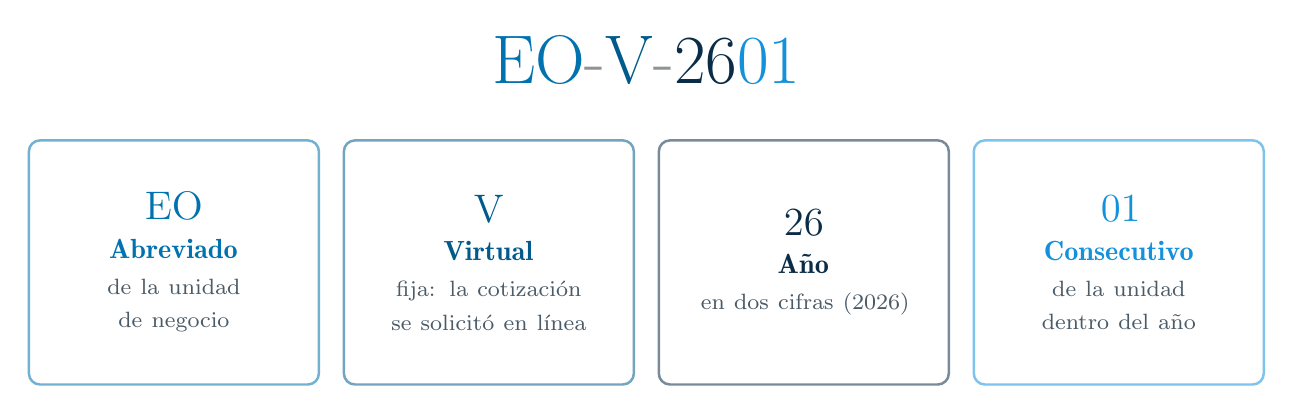
\begin{tikzpicture}
  \node[font=\montserrat\fontseries{eb}\selectfont\fontsize{40}{40}\selectfont] (c)
    {\textcolor{azul}{EO}\textcolor{grismarca}{-}\textcolor{azulhondo}{V}\textcolor{grismarca}{-}%
     \textcolor{noche}{26}\textcolor{azulvivo}{01}};
  \foreach \x/\col/\parte/\titulo/\texto in {
      -6.0/azul/EO/Abreviado/de la unidad de negocio,
      -2.0/azulhondo/V/Virtual/fija: la cotización se solicitó en línea,
      2.0/noche/26/Año/en dos cifras (2026),
      6.0/azulvivo/01/Consecutivo/de la unidad dentro del año} {
    \node[tarjeta, draw=\col!55, text width=3.05cm, minimum height=3.1cm, align=center, inner ysep=8pt, anchor=north] at (\x,-1.0)
      {{\color{\col}\montserrat\fontseries{eb}\selectfont\Large\parte}\\[2pt]
       {\fontseries{sb}\selectfont\color{\col}\titulo}\\[1pt]{\footnotesize\color{pizarra}\texto}};
  }
\end{tikzpicture}
\caption{Partes del código de cotización.}\label{fig:codigo}
\end{figure}

\begin{nota}
El consecutivo vuelve a empezar en 01 con la primera solicitud de cada año y tiene al menos
dos cifras: después de \texttt{EO-V-2699} sigue \texttt{EO-V-26100}. El abreviado de cada unidad
se define en \menu{Catálogo}{Unidades de negocio} (\seccion{sec:unidades}). En la instalación
actual, Auditoría usa \textbf{EO}, Consultoría usa \textbf{CNN} y Formación usa \textbf{GC}.
\end{nota}

\subsection{La lista de cotizaciones}\label{sec:lista-cotizaciones}

La pantalla \textbf{Cotizaciones} (\msg{Solicitudes recibidas desde el cotizador. Abra una para
subir la propuesta.}) muestra todas las solicitudes, con las más recientes arriba.

\begin{tabla}{colspec={Q[2.6cm,l] X[l]}}
  Columna & Qué muestra \\
  Código & El código de la solicitud. Haga clic en él para abrir el detalle. En pantallas
    pequeñas, la unidad y la fecha se muestran debajo del código. \\
  Cliente & Nombre del cliente y, debajo, su correo. \\
  Empresa & Razón social del cliente. Se oculta en pantallas pequeñas. \\
  Unidad & Unidad de negocio que eligió el cliente. \\
  Fecha & Fecha en que se recibió la solicitud. \\
  Estado & El estado de la solicitud (ver la tabla siguiente). \\
  Acciones & \icono[pizarra]{\icVer}\ Ver detalle y, si ya se envió la propuesta,
    \icono{\icExterno}\ Abrir propuesta. \\
\end{tabla}

\begin{tabla}{colspec={Q[3.2cm,l,m] X[l,m]}}
  Estado & Significado \\
  \pendiente & La solicitud llegó y todavía no se ha enviado la propuesta. \\
  \generada & Ya se envió la propuesta al cliente. \\
  \generada\ \novista & Se envió la propuesta, pero el cliente aún no la ha abierto. \\
  \generada\ \vista & El cliente abrió la propuesta desde el botón del correo. \\
\end{tabla}

La caja de búsqueda (\msg{Código, cliente o empresa…}) también encuentra solicitudes por el
correo, el NIT, el teléfono o el cargo del cliente, y por la unidad de negocio.

\captura[8cm]{03-01-cotizaciones-lista}{/dashboard/ordenes-cotizacion}{Lista de cotizaciones.}
  {la pantalla Cotizaciones con varias solicitudes, idealmente algunas en estado «Pendiente»
   y otras «Generada» con las insignias «Vista» o «No vista».}

\begin{consejo}
La lista no tiene filtro por estado. Para encontrar rápido las pendientes, fíjese en la columna
\campo{Estado}: las insignias \pendiente\ se distinguen por su color ámbar.
\end{consejo}

\subsection{Revisar una solicitud}\label{sec:detalle-cotizacion}

\begin{pasos}
  \item En la lista, haga clic en el \campo{Código} o en el ícono \icono[pizarra]{\icVer}
        \textbf{Ver detalle}.
  \item Se abre la pantalla \textbf{Cotización \var{código}}. Arriba a la izquierda está el
        botón \botonsec{\icAtras\ Volver a cotizaciones}. Debajo del título verá la fecha
        (\msg{Recibida el \var{dd/mm/aaaa}}) y el estado.
  \item Revise las tarjetas de la pantalla:
\end{pasos}

\begin{tabla}{colspec={Q[3cm,l] X[l]}}
  Tarjeta & Contenido \\
  Solicitud & La \campo{Unidad de negocio}. Las solicitudes antiguas, hechas antes del
    formulario de solicitud actual, muestran además la \campo{Línea de gestión} y los
    \campo{Servicios}. \\
  Respuestas (\var{N}) & Cada pregunta del formulario con la respuesta del cliente, en el
    orden en que la respondió. Si el cliente adjuntó archivos, en \campo{Adjuntar documentos}
    se ven solo sus nombres (\seccion{sec:documentos-cliente}). \\
  Cliente & \campo{Nombre} (enlace a la ficha del cliente), \campo{Correo}, \campo{Teléfono},
    \campo{Cargo}, \campo{Razón social}, \campo{NIT}, \campo{Actividad económica} y
        \campo{Dirección}. \\
\end{tabla}

\captura[9cm]{03-02-cotizacion-detalle}{/dashboard/ordenes-cotizacion/...}{Detalle de una solicitud pendiente.}
  {la pantalla de detalle de una solicitud en estado «Pendiente», con el botón «Enviar
   propuesta» arriba a la derecha y las tarjetas Solicitud, Respuestas y Cliente.}

\subsubsection{Documentos que adjunta el cliente}\label{sec:documentos-cliente}

El cliente puede adjuntar hasta 5 archivos por solicitud, de máximo 10 MB cada uno, en formato
PDF, Word, Excel, PowerPoint, JPG, PNG o ZIP. Training~InnovaQuote \textbf{no guarda esos archivos en el
panel}: los envía como archivos adjuntos en el correo \msg{Nueva solicitud de cotización
\var{código}} que recibe el \textbf{Correo de notificaciones} (\seccion{sec:configuracion}) y
los borra del servidor en cuanto el correo sale. En el detalle de la solicitud solo verá los
nombres de los archivos, en la respuesta \campo{Adjuntar documentos}.

\begin{importante}
Si el \campo{Correo de notificaciones} está vacío, los documentos del cliente se descartan y no
se puede recuperar ninguno. Mantenga siempre ese correo diligenciado y guarde los adjuntos
desde el buzón. Si el correo no llega a salir, los archivos pendientes se eliminan solos a las
24 horas.
\end{importante}

\subsection{Enviar la propuesta al cliente}\label{sec:enviar-propuesta}

La plataforma no guarda el archivo de la propuesta: guarda un \textbf{enlace} al documento.
Antes de empezar, suba la propuesta a un servicio de almacenamiento (por ejemplo, Google Drive,
OneDrive o SharePoint) y copie un enlace que el cliente pueda abrir sin iniciar sesión.

\begin{pasos}
  \item Abra la solicitud en estado \pendiente.
  \item Haga clic en \boton{\icCargar\ Enviar propuesta}, arriba a la derecha.
  \item Se abre la ventana \textbf{Enviar propuesta al cliente}, con el texto
        \msg{Pegue el enlace público del documento. El cliente recibirá un correo con un acceso
        seguro.}
  \item Pegue el enlace en \campo{URL de la propuesta}. Debe empezar por \texttt{https://} o
        \texttt{http://}.
  \item Haga clic en \boton{Guardar y notificar}. El botón se activa cuando el campo tiene
        texto y muestra \textbf{Enviando…} mientras procesa.
\end{pasos}

\captura[6.5cm]{03-03-enviar-propuesta}{/dashboard/ordenes-cotizacion/...}{Ventana para enviar la propuesta.}
  {la ventana «Enviar propuesta al cliente» abierta sobre el detalle de la solicitud, con un
   enlace de ejemplo pegado en «URL de la propuesta».}

\begin{resultado}
La ventana se cierra y aparece el aviso \msg{URL de cotización subida exitosamente.} El estado
cambia a \generada\ \insignianeutra{Aún no vista} y el botón de la esquina pasa a ser
\botonsec{\icExterno\ Abrir propuesta}.
\end{resultado}

\captura[8cm]{03-04-cotizacion-generada}{/dashboard/ordenes-cotizacion/...}{Solicitud después de enviar la propuesta.}
  {el detalle de la misma solicitud justo después de guardar, con el aviso de éxito, las
   insignias «Generada» y «Aún no vista», y el botón «Abrir propuesta».}

Al guardar, el sistema envía dos correos:

\begin{tabla}{colspec={Q[2.6cm,l] Q[5.2cm,l] X[l]}}
  Destinatario & Asunto & Contenido \\
  El cliente & \msg{Su cotización \var{código} está lista} & Le informa que la propuesta ya
    está disponible y trae el botón \textbf{Ver la cotización}, que la abre. Termina con los
    datos de contacto definidos en \seccion{sec:configuracion}. \\
  Correo de notificaciones & \msg{Cotización \var{código} generada (cliente notificado)} &
    Titulado \textbf{Cotización enviada al cliente}: confirma el envío con los datos del
    cliente y el botón \textbf{Abrir el documento}. Solo se envía si ese correo está
    configurado. \\
\end{tabla}

\begin{importante}
Revise el enlace antes de hacer clic en \boton{Guardar y notificar}: ábralo en una ventana de
incógnito para comprobar que el cliente podrá verlo. Una vez guardado, el panel no permite
cambiar ni borrar el enlace, y el correo al cliente ya habrá salido. Si se equivocó, contacte
al equipo técnico y envíe al cliente el enlace correcto por otro medio.
\end{importante}

Si el enlace no es válido, verá en rojo \msg{La URL de la cotización es obligatoria.} o
\msg{La URL debe ser una dirección válida.}

\subsection{Saber si el cliente vio la propuesta}\label{sec:vista}

La insignia \insigniainfo{Vista por el cliente} aparece la primera vez que el cliente abre la
propuesta con el botón \textbf{Ver la cotización} del correo. Mientras tanto, la solicitud
muestra \insignianeutra{Aún no vista} en el detalle y \novista\ en la lista.

\begin{nota}
Cuando usted hace clic en \botonsec{\icExterno\ Abrir propuesta}, el cliente no queda marcado
como si la hubiera visto. Tampoco cuenta si el cliente abre el documento por otro medio, por
ejemplo con un enlace que usted le compartió directamente.
\end{nota}

\section{Clientes}\label{sec:clientes}

\ficha{F2B9}{\menu{Operación}{Clientes}}{/dashboard/clientes}
  {Consultar quién ha cotizado, ver su historial y exportar la lista a Excel.}

Los clientes se registran solos cuando envían una solicitud desde Training~InnovaQuote. Cada cliente
se identifica por su correo: si alguien vuelve a cotizar con el mismo correo, se actualizan sus
datos y la nueva solicitud se suma a su historial.

\begin{nota}
Desde el panel no se pueden crear, editar ni eliminar clientes. Esta pantalla es de consulta.
\end{nota}

\subsection{La lista de clientes}

La pantalla \textbf{Clientes} (\msg{Personas que han solicitado cotizaciones, con su
historial.}) muestra primero a los clientes con la solicitud más reciente.

\begin{tabla}{colspec={Q[2.8cm,l] X[l]}}
  Columna & Qué muestra \\
  Cliente & Nombre (enlace a su ficha) y correo. \\
  Empresa & Razón social y, debajo, el cargo. \\
  Teléfono & Teléfono de contacto (se oculta en pantallas pequeñas). \\
  Cotizaciones & Total de solicitudes. Si tiene pendientes, aparece en ámbar
    \textbf{\var{N} pendiente(s)}. \\
  Última & Fecha de su solicitud más reciente (se oculta en pantallas pequeñas). \\
\end{tabla}

Para encontrar clientes puede combinar:

\begin{itemize}
  \item La búsqueda (\msg{Nombre, correo o empresa…}), que también encuentra por teléfono, NIT
        y cargo.
  \item El filtro \campo{Empresa}, con todas las razones sociales registradas.
  \item El filtro \campo{Unidad de negocio}, que muestra a los clientes con al menos una
        solicitud en esa unidad.
\end{itemize}

\captura[8cm]{03-05-clientes-lista}{/dashboard/clientes}{Lista de clientes con sus filtros.}
  {la pantalla Clientes con la búsqueda, los filtros «Empresa» y «Unidad de negocio», el botón
   verde «Exportar a Excel» y la tabla con varios clientes.}

\subsection{La ficha del cliente}

Haga clic en el nombre del cliente para abrir su ficha. Verá:

\begin{itemize}
  \item El nombre como título y, debajo, \textbf{\var{cargo} · \var{empresa}}.
  \item La tarjeta \textbf{Contacto}: \campo{Correo}, \campo{Teléfono}, \campo{Razón social},
        \campo{NIT}, \campo{Actividad económica}, \campo{Dirección}, \campo{Cargo} y
        \campo{Cliente desde} (fecha de su primera solicitud). Al hacer clic en el correo o el
        teléfono se abre su programa de correo o de llamadas.
  \item Los contadores \textbf{Cotizaciones}, \textbf{Generadas} y \textbf{Pendientes}.
  \item El \textbf{Historial de cotizaciones}, con las pestañas \textbf{Todas},
        \textbf{Generadas} y \textbf{Pendientes}, y una tabla con \campo{Código},
        \campo{Unidad}, \campo{Estado} y \campo{Fecha}. Haga clic en un código para abrir la
        solicitud.
\end{itemize}

\captura[9cm]{03-06-cliente-detalle}{/dashboard/clientes/...}{Ficha de un cliente con su historial.}
  {la ficha de un cliente que tenga más de una solicitud, mostrando la tarjeta Contacto, los
   contadores y el historial con sus pestañas.}

\subsection{Exportar los clientes a Excel}\label{sec:exportar}

\begin{pasos}
  \item Si solo quiere exportar una parte, aplique primero la búsqueda o los filtros. El archivo
        incluirá únicamente los resultados de la lista.
  \item Haga clic en \botonsec{{\color{verde}\icExcel}\ Exportar a Excel}, arriba a la
        derecha. Con una búsqueda o un filtro activo, el botón dice \textbf{Exportar resultados}.
  \item El botón muestra \textbf{Generando…} mientras se prepara el archivo. No cierre la
        página.
  \item Cuando el archivo está listo, el navegador lo descarga solo, con un nombre como
        \texttt{clientes\_03-11-2026\_08-02AM.xlsx}.
\end{pasos}

\begin{nota}
Si escribió algo en la búsqueda pero no presionó \tecla{Enter} ni \botonsec{Buscar}, ese texto
no se tiene en cuenta en la exportación.
\end{nota}

El archivo tiene una hoja llamada \textbf{Clientes} con el título \textbf{REPORTE DE CLIENTES},
la fecha de generación, el total de registros y el logo de Training Corporation. La tabla trae
estas columnas, con filtros en la cabecera, la cabecera fija al desplazarse y filas de color
alterno:

\begin{center}
\small
\begin{tabular}{@{}lll@{}}
  \textbullet\ ID & \textbullet\ Actividad económica & \textbullet\ Teléfono \\
  \textbullet\ Nombre & \textbullet\ Cargo & \textbullet\ Cotizaciones \\
  \textbullet\ Razón social & \textbullet\ Correo electrónico & \textbullet\ Última cotización \\
  \textbullet\ NIT & & \\
\end{tabular}
\end{center}

\capturaventana[7.5cm]{03-07-excel-clientes}{clientes\_03-11-2026\_08-02AM.xlsx}{Contenido del reporte de clientes exportado (hoja «Clientes»).}
  {solo el contenido de la hoja del archivo descargado, abierto en Excel o LibreOffice Calc,
   mostrando el título «REPORTE DE CLIENTES», el logo y las primeras filas.}

\begin{importante}
El enlace de descarga funciona una sola vez. Si necesita otra copia, vuelva a exportar. Los
archivos que no se descargan se borran del servidor a las 2 horas.
\end{importante}

Si algo falla, aparece un recuadro rojo debajo del encabezado:

\begin{tabla}{colspec={X[l] Q[5.6cm,l]}}
  Mensaje & Qué hacer \\
  \msg{No se pudo iniciar la exportación. Intente nuevamente.} & Vuelva a hacer clic en el botón. \\
  \msg{No se pudo generar el archivo. Intente nuevamente.} & Vuelva a intentar. Si se repite,
    avise al equipo técnico. \\
  \msg{Se perdió la conexión durante la exportación.} & Revise su conexión a internet y
    vuelva a exportar. \\
  \msg{La generación está tardando demasiado. Verifique que el worker de la cola esté en
    ejecución.} & El archivo se genera con un proceso en segundo plano del servidor. Avise al
    equipo técnico para que lo revise. \\
\end{tabla}

% =====================================================================
%  Capítulo 4 — Catálogo
% =====================================================================
\chapter{Catálogo}\label{cap:catalogo}

\entradilla{Lo que el cliente encuentra al cotizar: las unidades de negocio, su formulario de
preguntas y el catálogo de líneas de gestión y servicios.}

Los cuatro módulos del grupo \textbf{Catálogo} están relacionados entre sí, como muestra la
\figref{fig:relaciones}. Por eso conviene crearlos en este orden: primero las unidades de
negocio y las líneas de gestión, después los servicios y, por último, las preguntas de cada
unidad en el árbol de decisión.

\begin{figure}[H]
\centering
\begin{tikzpicture}[
    entidad/.style={tarjeta, minimum width=4.4cm, minimum height=1.35cm, text width=3.8cm, align=center},
    rel/.style={font=\scriptsize, text=pizarra, fill=white, inner sep=2pt},
  ]
  \node[entidad, draw=azul, line width=1.4pt] (u) at (0,0)
    {{\color{azul}\ico{F0B1}}\hspace{0.4em}\textbf{Unidad de negocio}\\{\scriptsize\color{pizarra}Tipo de servicio que elige el cliente}};
  \node[entidad] (a) at (-5.6,0)
    {{\color{azul}\ico{F0E8}}\hspace{0.4em}\textbf{Árbol de decisión}\\{\scriptsize\color{pizarra}Preguntas que responde el cliente}};
  \node[entidad] (s) at (5.6,0)
    {{\color{azul}\ico{F0AD}}\hspace{0.4em}\textbf{Servicios}\\{\scriptsize\color{pizarra}Oferta de cada unidad}};
  \node[entidad] (l) at (5.6,-2.4)
    {{\color{azul}\ico{F126}}\hspace{0.4em}\textbf{Línea de gestión}\\{\scriptsize\color{pizarra}Agrupa los servicios}};
  \draw[flecha] (u) -- node[rel, above=3pt] {tiene su propio} (a);
  \draw[flecha] (u) -- node[rel, above=3pt] {ofrece} (s);
  \draw[flecha] (l) -- node[rel, right=3pt] {clasifica} (s);
\end{tikzpicture}
\caption{Relación entre los módulos del catálogo.}\label{fig:relaciones}
\end{figure}

% ---------------------------------------------------------------------
\section{Unidades de negocio}\label{sec:unidades}

\ficha{F0B1}{\menu{Catálogo}{Unidades de negocio}}{/dashboard/unidad-negocio}
  {Crear, consultar, editar y eliminar las unidades de negocio.}

Cada unidad de negocio es un \textbf{tipo de servicio} que el cliente elige al entrar a Trainova, por ejemplo Auditoría, Consultoría o Formación. Cada unidad tiene su propio
formulario de preguntas y su propio consecutivo de códigos de cotización.

\begin{importante}
Una unidad solo aparece en Trainova cuando su árbol de decisión tiene al menos una
pregunta. Después de crear una unidad, configure sus preguntas (\seccion{sec:arbol}).
\end{importante}

\subsection{La lista de unidades}

La pantalla \textbf{Unidades de negocio} (\msg{Primer paso del cotizador. Cada unidad tiene su
propio árbol de decisión.}) muestra estas columnas:

\begin{tabla}{colspec={Q[3cm,l] X[l]}}
  Columna & Qué muestra \\
  ID & Número interno de la unidad. \\
  Nombre & Nombre de la unidad. Haga clic en él para ver su detalle. \\
  Abreviado & Prefijo de sus códigos de cotización, por ejemplo \textbf{EO}. \\
  Último código & El último código emitido, por ejemplo \textbf{EO-V-2603}, o
    \msg{sin cotizaciones aún}. \\
  Acciones & \icono[pizarra]{\icVer}\ Ver detalle, \icono{\icEditar}\ Editar y
    \icono[error]{\icEliminar}\ Eliminar. \\
\end{tabla}

La búsqueda (\msg{Nombre o abreviado…}) encuentra unidades por su nombre o por su abreviado.

\captura{04-01-unidades-lista}{/dashboard/unidad-negocio}{Lista de unidades de negocio.}
  {la pantalla Unidades de negocio con las unidades registradas y la columna «Último código».}

\subsection{Crear una unidad}\label{sec:unidad-crear}

\begin{pasos}
  \item Haga clic en \boton{\icMas\ Nueva unidad}.
  \item En \campo{Nombre}, escriba el nombre tal como lo verá el cliente, por ejemplo
        \textbf{Consultoría}.
  \item En \campo{Abreviado}, escriba entre 2 y 32 letras o números, sin espacios, por ejemplo
        \textbf{GA}. Las letras se convierten solas a mayúsculas.
  \item Haga clic en \boton{Crear unidad}.
\end{pasos}

\captura[7.5cm]{04-02-unidad-crear}{/dashboard/unidad-negocio/crear}{Formulario para crear una unidad de negocio.}
  {el formulario «Crear unidad de negocio» con los campos «Nombre» y «Abreviado» diligenciados
   con un ejemplo, antes de hacer clic en «Crear unidad».}

\begin{resultado}
Vuelve a la lista con el aviso \msg{La unidad de negocio «\var{nombre}» ha sido creada
exitosamente.} Para que los clientes puedan cotizarla, cree sus preguntas en el árbol de
decisión (\seccion{sec:arbol}).
\end{resultado}

\begin{tabla}{colspec={X[l] Q[6cm,l]}}
  Mensaje de error & Cómo resolverlo \\
  \msg{El nombre es obligatorio.} & Escriba un nombre. \\
  \msg{El nombre debe contener al menos una letra o número.} & El nombre no puede tener solo
    símbolos. \\
  \msg{Ya existe una unidad de negocio con un nombre equivalente.} & Ya hay una unidad con ese
    nombre, aunque cambien las tildes o las mayúsculas (por ejemplo, «Consultoría» y
    «consultoria»). Use otro nombre. \\
  \msg{El abreviado es obligatorio.} & Escriba un abreviado. \\
  \msg{Use al menos 2 caracteres en el abreviado.} & Alargue el abreviado. \\
  \msg{El abreviado solo puede incluir letras mayúsculas y números, sin espacios.} & Quite
    tildes, eñes, guiones y otros símbolos. \\
  \msg{Ese abreviado ya está en uso por otra unidad de negocio.} & Elija otro abreviado. \\
\end{tabla}

\subsection{Editar una unidad}\label{sec:unidad-editar}

\begin{pasos}
  \item En la fila de la unidad, haga clic en \icono{\icEditar} \textbf{Editar}.
  \item Cambie el \campo{Nombre} o el \campo{Abreviado}. Debajo de los campos verá, solo para
        consulta, el \textbf{Correlativo actual}, es decir, el último código emitido.
  \item Haga clic en \boton{Guardar cambios}.
\end{pasos}

\captura[7.5cm]{04-03-unidad-editar}{/dashboard/unidad-negocio/.../editar}{Edición de una unidad de negocio.}
  {el formulario «Editar unidad de negocio» de una unidad que ya tenga cotizaciones, para que
   se vea el recuadro «Correlativo actual».}

\begin{resultado}
Vuelve a la lista con el aviso \msg{La unidad de negocio «\var{nombre}» ha sido actualizada
exitosamente.}
\end{resultado}

\begin{importante}
\begin{itemize}
  \item \textbf{Cambiar el nombre cambia la dirección pública} del formulario de esa unidad. Si
        compartió con clientes un enlace directo al formulario, ese enlace dejará de funcionar.
  \item Evite renombrar una unidad mientras haya clientes llenando su formulario: la solicitud
        en curso podría fallar al enviarse.
  \item \textbf{Cambiar el abreviado solo afecta los códigos nuevos.} Las solicitudes anteriores
        conservan su código.
\end{itemize}
\end{importante}

\subsection{Ver el detalle de una unidad}

Haga clic en el nombre de la unidad o en \icono[pizarra]{\icVer} \textbf{Ver detalle}. La
pantalla muestra:

\begin{itemize}
  \item El nombre como título y, debajo, \textbf{Abreviado \var{ABREV} · último código
        \var{código}}.
  \item El botón \botonsec{\icEditar\ Editar}.
  \item La sección \textbf{Servicios (\var{N})}, con los servicios de la unidad. Haga clic en un
        servicio para editarlo. Si no tiene, verá \msg{Esta unidad no tiene servicios asociados.}
\end{itemize}

\captura[7cm]{04-04-unidad-detalle}{/dashboard/unidad-negocio/...}{Detalle de una unidad de negocio.}
  {la pantalla de detalle de una unidad con varios servicios en la tabla «Servicios».}

\subsection{Eliminar una unidad}

\begin{pasos}
  \item En la fila de la unidad, haga clic en \icono[error]{\icEliminar} \textbf{Eliminar}.
  \item Confirme el mensaje \msg{¿Eliminar la unidad «\var{nombre}»? También se borrará su árbol
        de decisión.}
\end{pasos}

Si la unidad tiene servicios, el sistema no la elimina y muestra \msg{No se puede eliminar la
unidad de negocio «\var{nombre}» porque tiene servicios asociados.} Elimine esos servicios o
asígnelos a otra unidad (\seccion{sec:servicios}) e intente de nuevo.

\begin{importante}
Al eliminar una unidad se borran también todas las preguntas de su árbol de decisión, y esto
no se puede deshacer. Las solicitudes que ya llegaron de esa unidad se conservan.
\end{importante}

% ---------------------------------------------------------------------
\section{Líneas de gestión}\label{sec:lineas}

\ficha{F126}{\menu{Catálogo}{Líneas de gestión}}{/dashboard/lineas-gestion}
  {Crear, editar y eliminar las líneas que agrupan los servicios.}

Las líneas de gestión agrupan los servicios por tema, por ejemplo HSEQ, Seguridad y Salud en
el Trabajo o Gestión Ambiental.

\subsection{La lista de líneas}

La tabla muestra \campo{ID}, \campo{Nombre} y \campo{Acciones} (\icono{\icEditar}\ Editar y
\icono[error]{\icEliminar}\ Eliminar). La búsqueda (\msg{Nombre o ID…}) encuentra líneas por
su nombre o número.

\captura[7cm]{04-05-lineas-lista}{/dashboard/lineas-gestion}{Lista de líneas de gestión.}
  {la pantalla Líneas de gestión con las líneas registradas.}

\subsection{Crear y editar una línea}

\begin{pasos}
  \item Haga clic en \boton{\icMas\ Nueva línea} o, para modificar una existente, en
        \icono{\icEditar} \textbf{Editar}.
  \item En \campo{Nombre}, escriba el nombre de la línea, por ejemplo \textbf{Calidad}. Debe ser
        único.
  \item Haga clic en \boton{Crear línea} o en \boton{Guardar cambios}.
\end{pasos}

\captura[5.5cm]{04-06-linea-crear}{/dashboard/lineas-gestion/crear}{Formulario para crear una línea de gestión.}
  {el formulario «Crear línea de gestión» con un nombre de ejemplo escrito.}

\begin{resultado}
Vuelve a la lista con el aviso \msg{Línea de gestión creada correctamente.} o
\msg{Línea de gestión actualizada exitosamente.}
\end{resultado}

Si el nombre ya existe, verá \msg{Ya existe una línea de gestión con ese nombre.}

\subsection{Eliminar una línea}

Haga clic en \icono[error]{\icEliminar} \textbf{Eliminar} y confirme
\msg{¿Eliminar la línea de gestión «\var{nombre}»?} Si la línea tiene servicios, el sistema no
la elimina y muestra \msg{No se puede eliminar la línea de gestión «\var{nombre}» porque tiene
servicios asociados.} Si se elimina, verá \msg{Línea de gestión eliminada exitosamente.}

% ---------------------------------------------------------------------
\section{Servicios}\label{sec:servicios}

\ficha{F0AD}{\menu{Catálogo}{Servicios}}{/dashboard/servicios}
  {Crear, editar y eliminar los servicios de cada unidad y línea de gestión.}

Cada servicio pertenece a una unidad de negocio y a una línea de gestión.

\begin{nota}
El catálogo de servicios sirve como referencia de la oferta de cada unidad. En la versión
actual de Trainova, el cliente describe su necesidad en el formulario de solicitud
(\seccion{sec:arbol}) y no elige servicios de esta lista. Las solicitudes antiguas que sí
incluían servicios los muestran en su detalle.
\end{nota}

\subsection{La lista de servicios}

La tabla muestra \campo{ID}, \campo{Nombre}, \campo{Unidad de negocio}, \campo{Línea de gestión}
y \campo{Acciones}. Puede combinar:

\begin{itemize}
  \item La búsqueda (\msg{Servicio o ID…}), que busca solo en el nombre del servicio o en su número.
  \item El filtro \campo{Unidad de negocio}, para ver los servicios de una sola unidad.
\end{itemize}

\captura[8cm]{04-07-servicios-lista}{/dashboard/servicios}{Lista de servicios filtrada por unidad.}
  {la pantalla Servicios con el filtro «Unidad de negocio» aplicado a una unidad.}

\subsection{Crear y editar un servicio}

\begin{pasos}
  \item Haga clic en \boton{\icMas\ Nuevo servicio} o, para modificar uno existente, en
        \icono{\icEditar} \textbf{Editar}.
  \item En \campo{Nombre}, escriba el nombre del servicio. No puede repetirse en ninguna otra
        unidad.
  \item En \campo{Unidad de negocio}, elija la unidad a la que pertenece.
  \item En \campo{Línea de gestión}, elija la línea que lo agrupa.
  \item Haga clic en \boton{Crear servicio} o en \boton{Guardar cambios}.
\end{pasos}

\captura[7cm]{04-08-servicio-crear}{/dashboard/servicios/crear}{Formulario para crear un servicio.}
  {el formulario «Crear servicio» con el nombre escrito y las listas «Unidad de negocio» y
   «Línea de gestión» con una opción elegida.}

\begin{resultado}
Vuelve a la lista con el aviso \msg{Servicio creado correctamente.} o
\msg{Servicio actualizado exitosamente.}
\end{resultado}

\begin{tabla}{colspec={X[l] Q[6cm,l]}}
  Mensaje & Cómo resolverlo \\
  \msg{Ya existe un servicio con ese nombre.} & Los nombres son únicos en todo el sistema. Use
    un nombre distinto. \\
  \msg{La unidad de negocio es obligatoria.} & Elija una unidad en la lista. \\
  \msg{La línea de gestión es obligatoria.} & Elija una línea en la lista. \\
  \msg{No existen unidades de negocio con las cuales usted pueda asociar un servicio.} & Cree
    primero una unidad (\seccion{sec:unidad-crear}). \\
  \msg{No existen líneas de gestión con las cuales usted pueda asociar un servicio.} & Cree
    primero una línea de gestión (\seccion{sec:lineas}). \\
\end{tabla}

\begin{consejo}
Para pasar un servicio a otra unidad o línea, edítelo y cambie la opción de la lista. Así puede
vaciar una unidad o una línea antes de eliminarla.
\end{consejo}

\subsection{Eliminar un servicio}

Haga clic en \icono[error]{\icEliminar} \textbf{Eliminar} y confirme
\msg{¿Eliminar el servicio «\var{nombre}»?} Verá el aviso \msg{Servicio eliminado exitosamente.}

% ---------------------------------------------------------------------
\section{Árbol de decisión}\label{sec:arbol}

\ficha{F0E8}{\menu{Catálogo}{Árbol de decisión}}{/dashboard/arbol-decision}
  {Diseñar el formulario de preguntas (formulario de solicitud) que responde el cliente de cada
   unidad.}

El árbol de decisión es el formulario que responde el cliente al cotizar: \msg{Las preguntas
que responde el cliente al cotizar, en el orden en que las verá.} Cada unidad de negocio tiene
el suyo.

\begin{importante}
Los cambios se aplican en Trainova apenas los guarda: no existe un paso de publicación.
Cada vez que guarda, el sistema comprueba que el cuestionario siga funcionando. Después de
cambios importantes, pruebe el formulario con \botonsec{\icPlay\ Probar como cliente}
(\seccion{sec:probar}).
\end{importante}

\subsection{Conceptos clave}\label{sec:conceptos-arbol}

\begin{tabla}{colspec={Q[3.4cm,l] X[l]}}
  Concepto & Qué es \\
  Pregunta & Cada campo que diligencia el cliente. \\
  Tipo de respuesta & Cómo responde el cliente: texto, número, fecha, documentos, una o
    varias opciones, o un rango (\seccion{sec:tipos-respuesta}). \\
  Opción & Cada alternativa de una pregunta de selección, por ejemplo «Presencial». \\
  Orden principal & La lista numerada de preguntas que todos los clientes recorren de arriba
    abajo. \\
  Pregunta de rama & Una pregunta adicional que solo aparece si el cliente elige cierta
    opción. Después, el cliente vuelve al orden principal. \\
  Bloque del formulario & El grupo temático en el que el cliente ve la pregunta. \\
\end{tabla}

La \figref{fig:ejemplo-arbol} muestra un ejemplo: la pregunta de sedes solo aparece cuando el
cliente elige una modalidad presencial o mixta.

\begin{figure}[H]
\centering
\begin{tikzpicture}[
    numero/.style={circle, fill=azul, text=white, minimum size=0.62cm, inner sep=0pt,
      font=\montserrat\bfseries\scriptsize},
    numerorama/.style={circle, draw=azulvivo, dashed, line width=1pt, text=azul, fill=white,
      minimum size=0.62cm, inner sep=0pt, font=\scriptsize},
    preg/.style={tarjeta, text width=6.4cm, font=\small},
    rama/.style={tarjeta, text width=5.2cm, font=\small, draw=azulvivo, dashed},
    etq/.style={font=\scriptsize, text=azulhondo, fill=white, inner sep=2pt},
  ]
  \node[preg, anchor=west] (q1) at (0.6,0)
    {\textbf{Modalidad de prestación del servicio}\\{\scriptsize\color{pizarra}Una opción: Presencial, Virtual, Mixto}};
  \node[numero] at (0,0) {1};
  \node[preg, anchor=west] (q2) at (0.6,-3.0)
    {\textbf{Descripción de horarios para la prestación del servicio}\\{\scriptsize\color{pizarra}Texto corto}};
  \node[numero] at (0,-3.0) {2};
  \node[preg, anchor=west] (q3) at (0.6,-4.8)
    {\textbf{Fecha estimada para la prestación del servicio}\\{\scriptsize\color{pizarra}Fecha}};
  \node[numero] at (0,-4.8) {3};
  \node[rama, anchor=west] (r1) at (9.9,-1.5)
    {\textbf{Descripción de sedes (lugar y dirección)}\\{\scriptsize\color{pizarra}Texto largo · pregunta de rama}};
  \node[numerorama] at (9.3,-1.5) {\ico{F149}};
  \draw[flecha] (q1.south) ++(-1.2,0) -- node[etq, left=2pt] {Virtual: sigue normal} ([xshift=-1.2cm]q2.north);
  \draw[flecha] (q1.east) -| node[etq, pos=0.25, above=2pt] {Presencial o Mixto} (9.3,-1.18);
  \draw[flecha] (r1.south) |- node[etq, pos=0.75, below=2pt] {después continúa en la 2} (q2.east);
  \draw[flecha] (q2.south) ++(-1.2,0) -- ([xshift=-1.2cm]q3.north);
\end{tikzpicture}
\caption{Ejemplo de árbol con una pregunta de rama.}\label{fig:ejemplo-arbol}
\end{figure}

El esquema está simplificado. En el formulario real, quien elige \textbf{Mixto} responde antes
dos preguntas sobre el tiempo del servicio en cada modalidad (presencial y virtual) y después
llega a la pregunta de sedes.

Los bloques del formulario agrupan las preguntas que ve el cliente. Son estos cuatro,
en este orden:

\begin{tabla}{colspec={Q[0.7cm,c] Q[5.4cm,l] X[l]}}
  N.º & Bloque & Lo que verá el cliente debajo del título \\
  1 & Identificación de la necesidad & Qué servicio requiere y cuáles son sus características. \\
  2 & Condiciones de prestación del servicio & Modalidad, lugar, horario, fecha y logística. \\
  3 & Información para la cotización & Insumos técnicos y económicos para estructurar la oferta. \\
    4 & Validación y cierre de la solicitud & Cómo resolver dudas antes de preparar la propuesta y cuándo espera recibirla. \\
\end{tabla}

Las preguntas sin bloque se muestran al cliente en un grupo llamado \textbf{Otras preguntas}.

\subsection{Elegir la unidad y leer el árbol}\label{sec:leer-arbol}

En la parte superior de la pantalla hay una pestaña por cada unidad de negocio, con su nombre y
el número de preguntas (por ejemplo, \textbf{24 preguntas}). Haga clic en una pestaña para ver
el árbol de esa unidad.

\captura[9.5cm]{04-09-arbol-vista-general}{/dashboard/arbol-decision}{Árbol de decisión de una unidad.}
  {la pantalla Árbol de decisión con las pestañas de las unidades arriba, el botón «Probar
   como cliente» y las primeras tarjetas de «Preguntas en orden», con los títulos azules de
   los bloques.}

La sección \textbf{Preguntas en orden} muestra el orden principal como una lista de tarjetas.
Cada tarjeta indica:

\begin{itemize}
  \item El número de la pregunta, en un círculo azul.
  \item El texto de la pregunta, en negrita, y debajo el tipo de respuesta y sus opciones.
  \item La etiqueta \insignianeutra{Opcional} si el cliente puede dejarla en blanco.
  \item Si alguna opción lleva a otra pregunta, líneas como \textbf{\icFlechaRama\ Si elige
        «Presencial» va a «Descripción de sedes…»} y \textbf{\icFlechaRama\ Con las demás
        opciones va a la pregunta 7}.
  \item A la derecha, los botones \icono{\icSubir} \textbf{Subir}, \icono{\icBajar}
        \textbf{Bajar} e \icono{\icEditar} \textbf{Editar}.
\end{itemize}

Si hay preguntas de rama, aparecen al final en la sección \textbf{Preguntas de rama}, sin número
y con el ícono \icono{\icFlechaRama}. Cada una indica cuándo aparece, por ejemplo
\msg{Aparece al elegir «Presencial» en la pregunta 9.}

El color del borde de cada tarjeta también informa:

\begin{tabla}{colspec={Q[3cm,l] X[l]}}
  Borde & Significado \\
  {\color{azul}\textbf{Azul}} & Es la pregunta que está editando. \\
  {\color{error}\textbf{Rojo}} & La pregunta tiene un problema, que se explica en rojo dentro de
    la tarjeta (\seccion{sec:validaciones-arbol}). \\
  {\color{ambartexto}\textbf{Ámbar}} & Es una pregunta de rama a la que ninguna opción lleva:
    \msg{Ninguna opción lleva aquí: el cliente no la verá.} \\
\end{tabla}

\subsection{Unidad sin preguntas: empezar o copiar}\label{sec:copiar-arbol}

Si la unidad aún no tiene preguntas verá \msg{«\var{unidad}» aún no tiene preguntas} y el
texto \msg{Sin preguntas, los clientes no pueden cotizar esta unidad. Empiece con la primera o
copie las de otra unidad.} Tiene dos caminos:

\begin{itemize}
  \item \boton{\icMas\ Crear la primera pregunta}: empieza un cuestionario desde cero
        (\seccion{sec:agregar-pregunta}).
  \item La lista \campo{Copiar las preguntas de…}: elija otra unidad y se copia de inmediato
        todo su cuestionario, con opciones, ramas y bloques. Verá el aviso
        \msg{Preguntas copiadas desde «\var{unidad}».}
\end{itemize}

\captura[6cm]{04-10-arbol-unidad-vacia}{/dashboard/arbol-decision}{Unidad sin preguntas, con la opción de copiar.}
  {la pestaña de una unidad sin preguntas, con el botón «Crear la primera pregunta» y la lista
   «Copiar las preguntas de…». Si todas las unidades tienen preguntas, cree una unidad de
   prueba para la captura y elimínela después.}

\begin{consejo}
Para crear el cuestionario de una unidad nueva, copie el de la unidad más parecida y ajústelo.
La copia solo está disponible mientras la unidad no tenga preguntas, así que nunca reemplaza un
cuestionario existente.
\end{consejo}

\subsection{Agregar una pregunta}\label{sec:agregar-pregunta}

Puede agregar preguntas en tres lugares de la lista:

\begin{itemize}
  \item \textbf{Insertar al inicio}, sobre la primera tarjeta.
  \item \textbf{Insertar pregunta aquí}, entre dos tarjetas. El botón se ve tenue y se resalta al
        pasar el ratón por el espacio entre ellas.
  \item \textbf{Añadir pregunta al final}, el botón punteado debajo de la última tarjeta.
\end{itemize}

\begin{pasos}
  \item Haga clic en el lugar donde quiere la pregunta. Se abre una tarjeta
        \textbf{Nueva pregunta}.
  \item Escriba el texto en \campo{Pregunta}.
  \item Complete los demás campos (ver la tabla siguiente).
  \item En \campo{¿Cómo responde el cliente?}, elija el tipo de respuesta
        (\seccion{sec:tipos-respuesta}).
  \item Si elige \textbf{Una opción} o \textbf{Varias opciones}, escriba las opciones
        (\seccion{sec:opciones}).
  \item Haga clic en \boton{Crear pregunta}.
\end{pasos}

\begin{tabla}{colspec={Q[4.4cm,l] X[l]}}
  Campo & Para qué sirve \\
  Pregunta & El texto que lee el cliente, por ejemplo \textit{¿Cuántos empleados tiene la
    empresa?} \\
  Ayuda para el cliente (opcional) & Una aclaración en letra pequeña que aparece debajo de la
    pregunta. \\
    Bloque del formulario & El bloque en el que aparecerá. Por defecto toma el de la pregunta vecina.
    Elija \textbf{Sin bloque} si no aplica. \\
  Opcional & Márquelo si el cliente puede dejar la pregunta en blanco y seguir. Sin marcar, la
    pregunta es obligatoria. \\
  ¿Cómo responde el cliente? & El tipo de respuesta. \\
  Ejemplo dentro del campo (opcional) & El texto gris de ejemplo dentro de la casilla, que
    desaparece al escribir. Solo para texto, número y fecha. \\
  Opciones & Las alternativas de las preguntas de selección. \\
\end{tabla}

\captura[10cm]{04-11-arbol-editar-pregunta}{/dashboard/arbol-decision}{Tarjeta de una pregunta abierta para editar.}
  {una tarjeta abierta en modo edición (borde azul), con los campos «Pregunta», «Ayuda para el
   cliente», «Bloque del formulario», «Opcional» y el inicio de «¿Cómo responde el cliente?».}

\begin{resultado}
La tarjeta se cierra, la pregunta aparece en su lugar y se muestra el aviso
\msg{Pregunta «\var{pregunta}» creada.}
\end{resultado}

\begin{nota}
Solo puede tener una pregunta abierta a la vez. El botón \boton{Crear pregunta} se mantiene
desactivado hasta que la pregunta esté completa; mientras tanto, un recuadro rojo dentro de la
tarjeta indica lo que falta.
\end{nota}

\subsection{Tipos de respuesta}\label{sec:tipos-respuesta}

\begin{tabla}{colspec={Q[3.3cm,l] Q[4.4cm,l] X[l]}}
  Tipo & Ejemplo en pantalla & Úselo para \\
  Una opción & Sí / No & Elegir una sola alternativa. Es el único tipo que permite ramas. \\
  Varias opciones & Marque todas las que apliquen & Marcar varias alternativas. \\
  Texto corto & Ente certificador & Respuestas de una línea. \\
  Texto largo & Descripción del servicio & Descripciones de varias líneas. \\
  Número & Cantidad de empleados & Cantidades. Solo admite números. \\
  Fecha & Fecha de inicio & Una fecha del calendario. \\
  Documentos & Adjuntar mapa de procesos & Archivos adjuntos: hasta 5, de máximo 10 MB cada uno. \\
  Rango de números & De 10 a 50 personas & Un valor inicial y uno final. \\
  Rango de fechas & Del 1 al 15 de marzo & Un periodo con fecha inicial y final. \\
\end{tabla}

\begin{nota}
En las preguntas de \textbf{Texto corto} y \textbf{Texto largo}, el cliente ve debajo de la
casilla un contador, por ejemplo \textbf{120 / 5.000 caracteres}: cada respuesta de texto admite
hasta 5.000 caracteres.
\end{nota}

\captura[6cm]{04-12-arbol-tipos-respuesta}{/dashboard/arbol-decision}{Selector del tipo de respuesta.}
  {un recorte de la cuadrícula «¿Cómo responde el cliente?» con los nueve tipos de respuesta.}

\subsection{Opciones de respuesta}\label{sec:opciones}

En las preguntas de tipo \textbf{Una opción} y \textbf{Varias opciones} aparece el editor de
\campo{Opciones}:

\begin{itemize}
  \item Escriba cada opción en su casilla. Presione \tecla{Enter} para crear la siguiente, o
        haga clic en \botonsec{Añadir opción}.
  \item Cambie el orden con \icono{\icSubir} \textbf{Subir opción} y \icono{\icBajar}
        \textbf{Bajar opción}.
  \item Quite una opción con \icono[error]{\icEliminar}. También puede presionar
        \tecla{Retroceso} en una opción vacía. Siempre debe quedar al menos una.
  \item Marque \campo{Incluir «Otro» para que escriba su respuesta} si quiere ofrecer una
        alternativa abierta. Se agrega la opción \textbf{Otro} al final; si el cliente la elige,
        aparece una casilla de texto con el ejemplo \msg{Especifique}.
\end{itemize}

\captura[8cm]{04-13-arbol-opciones}{/dashboard/arbol-decision}{Editor de opciones con ramas.}
  {el editor «Opciones» de una pregunta de tipo «Una opción» ya guardada, con varias opciones y
   la lista «Al elegirla» visible debajo de cada una.}

\subsection{Ramas: preguntas según la respuesta}\label{sec:ramas}

En las preguntas de \textbf{Una opción}, cada opción tiene debajo la lista \campo{Al elegirla},
que define a dónde va el cliente si la elige:

\begin{tabla}{colspec={Q[6.2cm,l] X[l]}}
  Opción de la lista & Qué hace \\
  Sigue normal (va a la pregunta \var{N}) & El cliente continúa con la siguiente pregunta del
    orden principal. Es la opción por defecto. \\
  Ir a: \var{N. pregunta} o Ir a: (rama) \var{pregunta} & Lleva al cliente a otra pregunta
    del orden principal o a una pregunta de rama ya creada. \\
  + Crear una pregunta solo para esta opción & Crea una pregunta de rama nueva que solo verá
    quien elija esta opción. \\
\end{tabla}

\subsubsection{Crear una pregunta de rama}

\begin{pasos}
  \item Guarde primero la pregunta con sus opciones. Mientras no esté guardada, la opción de
        crear aparece desactivada con el texto \msg{(guarde primero esta pregunta)} o
        \msg{(guarde primero los cambios)}.
  \item Abra de nuevo la pregunta haciendo clic en su tarjeta.
  \item Debajo de la opción, en \campo{Al elegirla}, elija
        \textbf{+ Crear una pregunta solo para esta opción}.
  \item Se abre la tarjeta \textbf{Nueva pregunta de rama} en la sección \textbf{Preguntas de
        rama}. Complétela como cualquier otra pregunta.
  \item Haga clic en \boton{Crear pregunta}.
\end{pasos}

\begin{resultado}
Quien elija esa opción verá la pregunta de rama y luego seguirá con la pregunta que venía
después en el orden principal.
\end{resultado}

\captura[8cm]{04-14-arbol-preguntas-rama}{/dashboard/arbol-decision}{Sección de preguntas de rama.}
  {la sección «Preguntas de rama» con al menos una tarjeta que muestre el texto «Aparece al
   elegir … en la pregunta …».}

Otras posibilidades de las ramas:

\begin{itemize}
  \item Varias opciones pueden llevar a la misma pregunta de rama. Por ejemplo, «Presencial» y
        «Mixto» pueden llevar a la pregunta de sedes eligiendo
        \textbf{Ir a: (rama) Descripción de sedes…}
  \item En una pregunta de rama ya creada, el campo \campo{Después de esta pregunta} define a
        dónde sigue el cliente: \textbf{Termina el cuestionario} o
        \textbf{Continúa en: \var{pregunta}}.
  \item Las preguntas de \textbf{Varias opciones} no pueden abrir ramas.
\end{itemize}

\begin{importante}
No envíe al cliente a una pregunta anterior: se formaría un ciclo del que el cliente nunca
saldría. El sistema lo detecta, muestra \msg{Se forma un ciclo: …} y no le deja guardar.
\end{importante}

\subsection{Editar, reordenar, duplicar y eliminar}\label{sec:editar-pregunta}

\subsubsection{Editar}

Haga clic en la tarjeta o en \icono{\icEditar} \textbf{Editar}, haga los cambios y luego clic en
\boton{Guardar pregunta}. Verá \msg{Pregunta «\var{pregunta}» guardada.} Para descartar los
cambios, haga clic en \botonsec{Cancelar}.

\subsubsection{Cambiar el orden}

Use \icono{\icSubir} \textbf{Subir} e \icono{\icBajar} \textbf{Bajar} en las tarjetas del
orden principal. La pregunta cambia de lugar con su vecina. No aparece un aviso: la lista se
actualiza sola. Las preguntas de rama no se reordenan, y las flechas se desactivan mientras
haya una pregunta abierta.

\subsubsection{Duplicar}

Con la pregunta abierta, haga clic en \botonsec{\icDuplicar\ Duplicar}. Se abre una copia
debajo, con el texto \textbf{\var{pregunta} (copia)} y las mismas opciones. Las ramas de las
opciones vuelven a \textbf{Sigue normal}. La copia no se guarda hasta que haga clic en
\boton{Crear pregunta}.

\begin{nota}
\botonsec{Duplicar} solo está disponible en el orden principal y sin cambios pendientes. Si
tiene cambios sin guardar, el botón muestra \msg{Guarde o cancele los cambios primero}.
\end{nota}

\subsubsection{Eliminar}

\begin{pasos}
  \item Abra la pregunta.
  \item Haga clic en \botonrojo{\icEliminar\ Eliminar}, abajo a la izquierda de la tarjeta.
  \item Confirme el mensaje \msg{¿Eliminar «\var{pregunta}»? Las preguntas siguientes se
        mantienen conectadas.}
\end{pasos}

Verá \msg{Pregunta «\var{pregunta}» eliminada.} El flujo no se rompe: lo que llevaba a la
pregunta eliminada ahora lleva a la siguiente.

\begin{importante}
Si la pregunta eliminada tenía opciones que abrían preguntas de rama, esas ramas no se borran:
quedan con borde ámbar y el mensaje \msg{Ninguna opción lleva aquí: el cliente no la verá.}
Vuelva a conectarlas desde una opción o elimínelas.
\end{importante}

\subsubsection{Cambios sin guardar}

Si tiene una pregunta abierta con cambios y trata de abrir otra, cambiar de pestaña o salir
de la pantalla, el sistema pregunta \msg{Tiene cambios sin guardar en la pregunta que está
editando. ¿Desea descartarlos?} Haga clic en \textbf{Cancelar} para volver y guardar, o en
\textbf{Aceptar} para descartar.

\subsection{Probar como cliente}\label{sec:probar}

\begin{pasos}
  \item Elija la pestaña de la unidad.
  \item Haga clic en \botonsec{\icPlay\ Probar como cliente}, arriba a la derecha.
  \item Se abre la ventana \textbf{Prueba: \var{unidad}}, con el aviso \msg{Así verá el cliente
        el formulario de solicitud. Nada de lo que responda aquí se guarda.}
  \item Responda el formulario como lo haría un cliente. Elija distintas opciones para comprobar
        que aparecen las preguntas de rama.
  \item Haga clic en \botonsec{Validar como al enviar}. Verá \msg{Todo listo para enviar.} o
        \msg{\var{N} campos por corregir.}, con el error en cada campo.
  \item Revise la sección \textbf{Así quedarán las respuestas en la cotización}: es lo que usted
        verá en el detalle de la solicitud.
  \item Cierre la ventana con la \textbf{\icCerrar}, la tecla \tecla{Esc} o haciendo clic fuera de ella.
\end{pasos}

\captura[9cm]{04-15-arbol-probar}{/dashboard/arbol-decision}{Ventana «Probar como cliente».}
  {la ventana «Prueba: …» abierta, con algunas respuestas diligenciadas y, si es posible, el
   resultado de «Validar como al enviar».}

\begin{nota}
La prueba usa la versión guardada del cuestionario. Si tiene una pregunta abierta con cambios,
guárdela antes de probar.
\end{nota}

\subsection{Mensajes de validación}\label{sec:validaciones-arbol}

Estos mensajes aparecen en rojo dentro de la tarjeta, o como alerta general sobre la lista:

\begin{tabla}{colspec={Q[5.4cm,l] X[l]}}
  Mensaje & Qué significa y cómo resolverlo \\
  \msg{Escriba la pregunta.} & El texto de la pregunta está vacío. Escríbalo. \\
  \msg{Agregue al menos una opción.} & La pregunta de selección no tiene opciones. La opción
    «Otro» sola no cuenta. \\
  \msg{Hay opciones sin texto: escríbalas o quítelas.} & Alguna casilla de opción está vacía. \\
  \msg{Lleva a una pregunta que ya no existe.} & Una opción o el campo «Después de esta
    pregunta» apunta a una pregunta eliminada. Elija otro destino. \\
  \msg{Se forma un ciclo: «A» → «B» → «A». El cliente nunca terminaría.} & Un destino devuelve
    al cliente a una pregunta anterior. Elija una pregunta posterior o \textbf{Sigue normal}. \\
  \msg{El cuestionario no tiene una primera pregunta.} & El cuestionario perdió su punto de
    inicio. Agregue una pregunta con \textbf{Insertar al inicio}; si el mensaje no desaparece,
    avise al equipo técnico. \\
  \msg{Ninguna opción lleva aquí: el cliente no la verá.} & Pregunta de rama sin uso.
    Conéctela desde una opción o elimínela. \\
\end{tabla}

\captura[6cm]{04-16-arbol-validacion}{/dashboard/arbol-decision}{Recuadro con los problemas de una pregunta.}
  {una tarjeta abierta con el recuadro rojo de problemas, por ejemplo una pregunta nueva de
   tipo «Una opción» con una opción vacía. Haga clic en «Cancelar» después de capturarla.}

\subsection{Buenas prácticas}

\begin{itemize}
  \item Escriba preguntas cortas y claras. Use \campo{Ayuda para el cliente} para las
        aclaraciones y \campo{Ejemplo dentro del campo} para mostrar el formato esperado.
  \item Asigne cada pregunta a su bloque, para que el cliente vea un formulario ordenado.
  \item Marque como \campo{Opcional} solo lo que de verdad no es necesario para cotizar.
  \item Después de cada cambio importante, use \botonsec{\icPlay\ Probar como cliente}.
  \item Haga los cambios grandes en horarios de poco movimiento: se aplican de inmediato.
  \item Revise que no queden preguntas de rama con borde ámbar.
  \item Auditoría y Consultoría deben mantener el mismo formulario (solo cambian los ejemplos
        dentro de los campos). Si cambia una pregunta, sus opciones, su orden o si es
        obligatoria en una de las dos unidades, haga el mismo cambio en la otra. Formación no
        sigue esta regla.
\end{itemize}

% =====================================================================
%  Capítulo 5 — Sistema
% =====================================================================
\chapter{Sistema: usuarios, correos y configuración}\label{cap:sistema}

\entradilla{Las cuentas con acceso al panel, las invitaciones a clientes y los datos que
acompañan los correos de la plataforma.}

% ---------------------------------------------------------------------
\section{Usuarios}\label{sec:usuarios}

\ficha{F0C0}{\menu{Sistema}{Usuarios}}{/dashboard/usuarios}
  {Crear, editar y eliminar las cuentas con acceso al panel.}

\begin{importante}
Todas las cuentas tienen acceso completo al panel, como se explica en la
\seccion{sec:quien}. Antes de crear una cuenta, asegúrese de que la persona deba administrar
Training~InnovaQuote.
\end{importante}

\subsection{La lista de usuarios}

La pantalla \textbf{Usuarios} (\msg{Cuentas con acceso al panel de administración.}) muestra
\campo{ID}, \campo{Nombre}, \campo{Correo}, \campo{Teléfono} y \campo{Acciones}. Su propia
cuenta aparece marcada con \textbf{(usted)} junto al nombre y no tiene ícono de eliminar. La búsqueda (\msg{Nombre o correo…}) encuentra usuarios por su nombre o su correo.

\captura[7cm]{05-01-usuarios-lista}{/dashboard/usuarios}{Lista de usuarios del panel.}
  {la pantalla Usuarios con al menos dos cuentas, en la que se vea la marca «(usted)» en su fila.}

\subsection{Crear un usuario}\label{sec:usuario-crear}

\begin{pasos}
  \item Haga clic en \boton{\icMas\ Nuevo usuario}. Se abre \textbf{Crear usuario}, con el aviso
        \msg{Las cuentas de usuario tienen acceso completo al panel.}
  \item Complete los campos:
\end{pasos}

\begin{tabla}{colspec={Q[3.8cm,l] X[l]}}
  Campo & Qué escribir \\
  Nombre & Nombre completo de la persona. El Panel de inicio la saludará por el primer nombre. \\
  Correo electrónico & El correo con el que iniciará sesión. No puede estar registrado en otra
    cuenta. \\
  Teléfono & Entre 10 y 15 caracteres, por ejemplo \texttt{3001234567}. \\
  Contraseña & Mínimo 8 caracteres. \\
\end{tabla}

\begin{pasos}[resume]
  \item Haga clic en \boton{Crear usuario}.
\end{pasos}

\captura[7.5cm]{05-02-usuario-crear}{/dashboard/usuarios/crear}{Formulario para crear un usuario.}
  {el formulario «Crear usuario» con datos de ejemplo. No muestre una contraseña real: el
   campo la oculta, pero use una de prueba.}

\begin{resultado}
Vuelve a la lista con el aviso \msg{Usuario creado correctamente.} La persona ya puede iniciar
sesión (\seccion{sec:iniciar-sesion}).
\end{resultado}

\begin{consejo}
Entregue la contraseña inicial por un medio seguro, nunca en el mismo mensaje que el correo de
acceso, y pídale a la persona que la cambie en su primer ingreso. Cada usuario puede cambiar su
propia contraseña editando su fila en \menu{Sistema}{Usuarios}.
\end{consejo}

\begin{tabla}{colspec={X[l] Q[6cm,l]}}
  Mensaje & Cómo resolverlo \\
  \msg{El nombre es obligatorio} & Escriba el nombre. \\
  \msg{El correo es obligatorio} / \msg{El correo debe ser válido} & Escriba un correo con la
    forma \texttt{nombre@empresa.com}. \\
  \msg{Este correo ya está registrado} & Ya existe una cuenta con ese correo. Búsquela en la
    lista. \\
  \msg{La contraseña es obligatoria} / \msg{La contraseña debe tener al menos 8 caracteres} &
    Escriba una contraseña más larga. \\
  \msg{El teléfono es obligatorio} / \msg{El teléfono debe tener al menos 10 dígitos} /
    \msg{El teléfono no puede tener más de 15 dígitos} & Revise la longitud del teléfono. \\
\end{tabla}

\subsection{Editar un usuario y cambiar su contraseña}\label{sec:usuario-editar}

\begin{pasos}
  \item En la fila del usuario, haga clic en \icono{\icEditar} \textbf{Editar}. El título es
        \textbf{Editar usuario} y debajo aparece su correo.
  \item Cambie los datos que necesite.
  \item Para asignar una contraseña nueva, escríbala en \campo{Nueva contraseña}. Si deja el
        campo vacío, se conserva la actual (\msg{Déjela en blanco para conservar la actual.}).
  \item Haga clic en \boton{Guardar cambios}.
\end{pasos}

\captura[7.5cm]{05-03-usuario-editar}{/dashboard/usuarios/.../editar}{Edición de un usuario.}
  {el formulario «Editar usuario», en el que se vea el campo «Nueva contraseña (opcional)» con
   su texto de ayuda.}

\begin{resultado}
Vuelve a la lista con el aviso \msg{Usuario actualizado correctamente.}
\end{resultado}

\subsection{Eliminar un usuario}

\begin{pasos}
  \item En la fila del usuario, haga clic en \icono[error]{\icEliminar} \textbf{Eliminar}.
  \item Confirme el mensaje \msg{¿Eliminar al usuario \var{nombre}?}
\end{pasos}

Verá el aviso \msg{Usuario eliminado correctamente.} La persona pierde el acceso al panel de
inmediato.

\begin{nota}
No puede eliminar su propia cuenta: su fila no tiene el ícono y, si lo intentara, el sistema
respondería \msg{No puedes eliminar tu propio usuario.} Si necesita retirar su acceso, pídaselo
a otro administrador.
\end{nota}

% ---------------------------------------------------------------------
\section{Correos de bienvenida}\label{sec:bienvenida}

\ficha{F0E0}{\menu{Sistema}{Correos de bienvenida}}{/dashboard/correos-bienvenida}
  {Invitar clientes a usar la plataforma con un correo de bienvenida.}

Este módulo envía un correo que presenta Training~InnovaQuote a una lista de direcciones. El subtítulo de
la pantalla indica a dónde lleva el botón del correo: \msg{Invite a sus clientes a la
plataforma. El botón del correo lleva a la página para solicitar una cotización:
\var{dirección}.} Esa dirección es la de la página de solicitud, \ruta{\dominio\allowbreak/cotizar}.

\begin{pasos}
  \item Prepare la lista de correos. Puede copiar directamente la columna de correos de una hoja
        de cálculo.
  \item Pegue la lista en \campo{Lista de correos}. Separe las direcciones con un salto de
        línea, una coma (,), un punto y coma (;) o una barra vertical (\textbar).
  \item Revise el contador debajo de la caja: \msg{\var{N} correos únicos detectados · máximo
        500 por envío}. Los correos repetidos se cuentan una sola vez. Si pasa de 500, el número
        se pone en rojo.
  \item Haga clic en \boton{\icEnviar\ Poner en cola el envío}.
\end{pasos}

\captura[8cm]{05-04-correos-bienvenida}{/dashboard/correos-bienvenida}{Envío de correos de bienvenida.}
  {la pantalla Correos de bienvenida con dos o tres correos de prueba escritos en «Lista de
   correos» y el contador de correos detectados. Use correos de prueba, no de clientes reales.}

\begin{resultado}
Verá el aviso \msg{Se pusieron en cola \var{N} correos de bienvenida.} Si algunas líneas no
eran correos válidos, el aviso agrega \msg{Se omitieron \var{X} líneas sin correo válido (ej.:
…).} La caja se vacía sola para que no envíe la misma lista dos veces.
\end{resultado}

\begin{tabla}{colspec={Q[6.2cm,l] Q[2.2cm,c] X[l]}}
  Ejemplo de línea & ¿Sirve? & Observación \\
  \texttt{cliente@empresa.com} & Sí & Formato correcto. \\
  \texttt{Cliente@Empresa.COM} & Sí & Se convierte a minúsculas. \\
  \texttt{a@empresa.com; b@empresa.com} & Sí & Separados por punto y coma. \\
  \texttt{a@empresa.com b@empresa.com} & No & El espacio no separa direcciones. \\
  \texttt{Ana Pérez <ana@empresa.com>} & No & No incluya el nombre junto al correo. \\
\end{tabla}

El correo que recibe cada persona:

\begin{itemize}
  \item \textbf{Asunto:} \msg{Hemos lanzado una nueva plataforma para cotizaciones}.
  \item \textbf{Título:} \msg{Cotice en línea con Training Corporation}.
  \item \textbf{Saludo:} \msg{Estimado/a cliente:}, seguido de un texto que explica que ahora
        puede elegir el servicio, diligenciar el formulario de solicitud y recibir la propuesta
        en su correo.
  \item \textbf{Botón:} \textbf{Solicitar una cotización}, que lleva a la página de solicitud de
        Training~InnovaQuote.
  \item \textbf{Cierre:} la firma \msg{Cordialmente, Equipo de Training Corporation} y, al pie,
        los datos de contacto definidos en \menu{Sistema}{Configuración}.
\end{itemize}

\begin{importante}
Cada envío manda un correo a cada dirección de la lista, aunque ya la haya invitado antes. Lleve
un control de a quién invitó. Los correos se envían en segundo plano y pueden tardar unos
minutos en llegar.
\end{importante}

\begin{tabla}{colspec={X[l] Q[5.6cm,l]}}
  Mensaje de error & Cómo resolverlo \\
  \msg{Indique al menos una dirección de correo electrónico.} & La caja está vacía. \\
  \msg{No se encontró ningún correo válido. Verifique el formato (ejemplo: nombre@empresa.com).}
    & Revise los separadores y quite los nombres. \\
  \msg{Máximo 500 correos por envío. Reduzca la lista e intente nuevamente.} & Divida la lista
    en grupos de 500 o menos. \\
\end{tabla}

% ---------------------------------------------------------------------
\section{Configuración}\label{sec:configuracion}

\ficha{F013}{\menu{Sistema}{Configuración}}{/dashboard/configuraciones}
  {Definir quién recibe las notificaciones y los datos de contacto de los correos.}

La pantalla \textbf{Configuración} (\msg{Destinatario de las notificaciones y datos de contacto
que aparecen en los correos al cliente.}) tiene dos secciones. Todos los campos son opcionales.

\begin{tabla}{colspec={Q[4.2cm,l] X[l]}}
  Campo & Para qué sirve \\
  \SetCell[c=2]{l, bg=nube} \textbf{Notificaciones} & \\
  Correo de notificaciones & Recibe el aviso \msg{Nueva solicitud de cotización \var{código}}
    con cada solicitud, \textbf{junto con los documentos que adjuntó el cliente}, y el aviso
    \msg{Cotización \var{código} generada (cliente notificado)} con cada propuesta enviada. Si
    lo deja vacío, no se envían estos avisos y los documentos del cliente se pierden
    (\seccion{sec:documentos-cliente}). \\
  \SetCell[c=2]{l, bg=nube} \textbf{Datos de contacto (pie de los correos)} & \\
  Correo de contacto & El correo al que pueden escribir los clientes. \\
  Teléfono & El teléfono de contacto. \\
  URL del sitio web & La dirección del sitio web, completa, por ejemplo
    \texttt{https://www.trainingcorporation.com.co}. \\
  Texto del enlace & El texto visible del enlace al sitio web. Si lo deja vacío, se muestra la
    dirección. \\
  Dirección & La dirección física de la empresa. \\
\end{tabla}

Los datos de contacto aparecen al pie de todos los correos que recibe el cliente (solicitud
pendiente, propuesta lista y bienvenida), bajo el texto \msg{¿Tiene preguntas? Llame o escriba}. Los campos vacíos no se muestran.

\begin{pasos}
  \item Complete o cambie los campos.
  \item Haga clic en \boton{Guardar configuración}.
\end{pasos}

\captura[9cm]{05-05-configuracion}{/dashboard/configuraciones}{Pantalla de configuración.}
  {la pantalla Configuración completa, con las secciones «Notificaciones» y «Datos de contacto
   (pie de los correos)» diligenciadas.}

\begin{resultado}
Verá el aviso \msg{Configuración actualizada exitosamente.} Los cambios se aplican a los
correos que salgan desde ese momento.
\end{resultado}

\begin{nota}
Esta pantalla no tiene botón \botonsec{Cancelar}. Si no quiere guardar lo que cambió, salga de
la pantalla sin hacer clic en \boton{Guardar configuración}.
\end{nota}

\begin{tabla}{colspec={X[l] Q[5.6cm,l]}}
  Mensaje de error & Cómo resolverlo \\
  \msg{El correo de notificaciones debe ser una dirección válida.} & Revise el formato del
    correo. \\
  \msg{El correo de contacto debe ser una dirección válida.} & Revise el formato del correo. \\
  \msg{La URL del sitio web debe ser una dirección válida (https://…).} & Escriba la dirección
    completa, empezando por \texttt{https://}. \\
\end{tabla}

% =====================================================================
%  Capítulo 6 — Ver el sitio público y cerrar sesión
% =====================================================================
\chapter{Ver el sitio y cerrar sesión}\label{cap:salida}

\entradilla{El final del recorrido: comprobar lo que ve el cliente y salir del panel de forma
segura.}

\section{Ver el sitio público}\label{sec:sitio-publico}

Al final de la barra lateral, \textbf{\icExterno\ Ver sitio público} abre la página de inicio de Training~InnovaQuote en una pestaña nueva. El panel sigue abierto en la pestaña original.

Úselo para comprobar sus cambios desde el punto de vista del cliente. Por ejemplo:

\begin{itemize}
  \item Que una unidad de negocio nueva aparezca en \msg{Elija el tipo de servicio}, después de
        crear sus preguntas.
  \item Que el formulario de una unidad muestre las preguntas y los bloques en el orden
        esperado.
\end{itemize}

\captura[8cm]{06-01-sitio-publico}{/}{Página de inicio de Training~InnovaQuote.}
  {la página de inicio pública de Training~InnovaQuote, abierta desde «Ver sitio público».}

\begin{importante}
Si envía una solicitud de prueba desde el sitio público, se creará una cotización real con su
código y llegarán los correos de confirmación. Para revisar el formulario sin crear solicitudes,
use \botonsec{\icPlay\ Probar como cliente} (\seccion{sec:probar}).
\end{importante}

\section{Cerrar sesión}\label{sec:cerrar-sesion}

\begin{pasos}
  \item Guarde lo que esté editando. Por ejemplo, en el árbol de decisión, termine con
        \boton{Guardar pregunta} o \botonsec{Cancelar}.
  \item Vaya al final de la barra lateral. En un celular, abra antes el menú con
        \textbf{\icMenu} (\seccion{sec:movil}).
  \item Debajo de \textbf{Ver sitio público} verá \textbf{\icSalir\ Cerrar sesión}, con el
        correo de su cuenta.
  \item Haga clic en \textbf{Cerrar sesión}.
\end{pasos}

\capturaconnotas[6.5cm]{06-02-cerrar-sesion}{/dashboard}{Opción «Cerrar sesión» al final de la barra lateral.}
  {un recorte de la parte inferior de la barra lateral, con «Ver sitio público», «Cerrar
   sesión» y el correo de la cuenta.}
  {\textbf{Antes de salir}

   \begin{itemize}
     \item Compruebe que el último aviso fue de éxito.
     \item Si dejó una pregunta abierta en el árbol de decisión, guárdela o cancélela: al cerrar
           sesión, el sistema no le avisa y los cambios sin guardar se pierden.
     \item El correo bajo \textbf{Cerrar sesión} le confirma con qué cuenta está trabajando.
   \end{itemize}}

\begin{resultado}
La sesión se cierra y el navegador lo lleva a la página de inicio pública de Training~InnovaQuote. Para
volver a entrar, siga los pasos de la \seccion{sec:iniciar-sesion}.
\end{resultado}

\begin{consejo}
\begin{itemize}
  \item Cierre sesión siempre que use un computador compartido. Cerrar la pestaña o el
        navegador no basta, sobre todo si marcó \campo{Mantener la sesión iniciada}.
  \item Si deja el panel sin usar por un tiempo largo (por defecto, 2 horas), la sesión se
        cierra sola y deberá iniciar sesión de nuevo. Si estaba llenando un formulario, podría
        perder lo que escribió.
\end{itemize}
\end{consejo}

\newcommand{\caprefclaro}[1]{\hyperref[#1]{\textcolor{cielo}{\fontseries{sb}\selectfont capítulo~\ref*{#1}}}}

\begin{tcolorbox}[enhanced, colback=noche, colframe=noche, coltext=white, arc=6pt,
    left=16pt, right=16pt, top=14pt, bottom=14pt, before skip=18pt,
    overlay={\begin{scope}
        \clip (frame.south west) rectangle (frame.north east);
        \pic[opacity=0.35] at ([xshift=-1.6cm, yshift=-0.3cm]frame.north east) {anillo={2.6cm/1.2pt/cielo}};
      \end{scope}}]
  {\montserrat\bfseries\large\color{white}Recorrido completo}\par\vspace{4pt}
  {\color{niebla}Ya conoce el flujo completo del administrador:}\par\vspace{6pt}
  \begin{itemize}[label={\color{cielo}\ico{F00C}}, leftmargin=1.6em]
    \item Iniciar sesión y recuperar la contraseña (\caprefclaro{cap:acceso}).
    \item Revisar solicitudes, enviar propuestas y consultar clientes (\caprefclaro{cap:operacion}).
    \item Mantener el catálogo y el árbol de decisión (\caprefclaro{cap:catalogo}).
    \item Administrar usuarios, invitaciones y configuración (\caprefclaro{cap:sistema}).
    \item Revisar el sitio público y cerrar sesión (\caprefclaro{cap:salida}).
  \end{itemize}
\end{tcolorbox}

% =====================================================================
%  Capítulo 7 — Capacidad de la aplicación
% =====================================================================
\chapter{Capacidad de la aplicación}\label{cap:capacidad}

\entradilla{Cuántas personas pueden usar Training~InnovaQuote al mismo tiempo manteniendo una buena
experiencia.}

Los \textbf{usuarios simultáneos} son las personas que están usando Training~InnovaQuote en el mismo
momento, por ejemplo navegando por el sitio o llenando el formulario de solicitud. No es lo
mismo que el total de visitas del día.

\begin{tcolorbox}[enhanced, colback=nube, colframe=nube, arc=6pt, left=16pt, right=16pt,
    top=13pt, bottom=13pt, before skip=12pt, after skip=14pt, borderline west={3.5pt}{0pt}{azul}]
  {\montserrat\bfseries\color{azul}{\iconos\char"F0C0\relax}\hspace{0.55em}En resumen}\par\vspace{5pt}
  Con \textbf{50 usuarios simultáneos} navegando y llenando el formulario, Training~InnovaQuote responde en
  \textbf{menos de 0,35 segundos el 95 \% de las veces} y sin errores. Mantiene una buena
  experiencia hasta unos \textbf{100 usuarios}, empieza a ponerse lenta cerca de \textbf{200} y se
  satura sobre los \textbf{300}.

  \vspace{4pt}
  Funciona en una máquina de \textbf{2 vCPU y 4 GB de memoria}. Si se necesita más capacidad, se
  amplía subiendo el tamaño de la máquina.
\end{tcolorbox}

\definecolor{ambarvivo}{HTML}{E8A317}
\begin{figure}[H]
\centering
\begin{tikzpicture}[
    marca/.style={circle, fill=white, draw=noche, line width=1.4pt, minimum size=0.38cm, inner sep=0pt},
    cifra/.style={font=\montserrat\fontseries{eb}\selectfont\large, text=noche},
    texto/.style={font=\footnotesize, text=pizarra, text width=3.2cm, align=center},
  ]
  % Barra: de 0 a 350 usuarios en 15 cm
  \begin{scope}
    \clip[rounded corners=0.22cm] (0,-0.22) rectangle (15,0.22);
    \shade[left color=verde, right color=ambarvivo] (0,-0.22) rectangle (8.57,0.22);
    \shade[left color=ambarvivo, right color=error] (8.57,-0.22) rectangle (15,0.22);
  \end{scope}
  \foreach \x/\n/\desc in {2.14/50/{Responde en menos de 0,35 s, sin errores}, 8.57/200/{Empieza a ponerse lenta}} {
    \node[marca] at (\x,0) {};
    \node[cifra, anchor=north] (c) at (\x,-0.42) {\n};
    \node[texto, anchor=north] at (c.south) {\desc};
  }
  \foreach \x/\n/\desc in {4.29/100/{Buena experiencia hasta aquí}, 12.86/300/{Se satura}} {
    \node[marca] at (\x,0) {};
    \node[cifra, anchor=south] (c) at (\x,0.42) {\n};
    \node[texto, anchor=south] at (c.north) {\desc};
  }
  \node[font=\scriptsize, text=pizarra, anchor=north east] at (15,-0.35) {usuarios simultáneos};
\end{tikzpicture}
\caption{Comportamiento de Training~InnovaQuote según el número de usuarios simultáneos.}\label{fig:capacidad}
\end{figure}

\begin{resultado}[Conclusión]
Training~InnovaQuote atiende \textbf{50 usuarios simultáneos} con una holgura de unas \textbf{2 a 3 veces}.
\end{resultado}


\appendix
\apendicestrue
% =====================================================================
%  Apéndices
% =====================================================================
\chapter{Mensajes del sistema}\label{ap:mensajes}

\entradilla{Referencia rápida de los avisos que muestra el panel después de cada acción,
agrupados por módulo.}

\begin{longtblr}{colspec={Q[3.1cm,l] X[l] Q[4.2cm,l]}}
  Módulo & Mensaje & Cuándo aparece \\
  Cotizaciones & \msg{URL de cotización subida exitosamente.} & Al enviar la propuesta. \\
  Cotizaciones & \msg{La URL de la cotización es obligatoria.} & Al enviar sin enlace. \\
  Cotizaciones & \msg{La URL debe ser una dirección válida.} & El enlace no tiene formato de dirección web. \\
  Clientes & \msg{No se pudo iniciar la exportación. Intente nuevamente.} & Falla al iniciar el Excel. \\
  Clientes & \msg{No se pudo generar el archivo. Intente nuevamente.} & Falla al generar el Excel. \\
  Clientes & \msg{Se perdió la conexión durante la exportación.} & Se cortó internet mientras se generaba. \\
  Clientes & \msg{La generación está tardando demasiado. Verifique que el worker de la cola esté en ejecución.} & El proceso en segundo plano no responde. \\
  Unidades de negocio & \msg{La unidad de negocio «\var{nombre}» ha sido creada exitosamente.} & Al crear. \\
  Unidades de negocio & \msg{La unidad de negocio «\var{nombre}» ha sido actualizada exitosamente.} & Al editar. \\
  Unidades de negocio & \msg{La unidad de negocio «\var{nombre}» ha sido eliminada exitosamente.} & Al eliminar. \\
  Unidades de negocio & \msg{No se puede eliminar la unidad de negocio «\var{nombre}» porque tiene servicios asociados.} & Al eliminar una unidad con servicios. \\
  Líneas de gestión & \msg{Línea de gestión creada correctamente.} & Al crear. \\
  Líneas de gestión & \msg{Línea de gestión actualizada exitosamente.} & Al editar. \\
  Líneas de gestión & \msg{Línea de gestión eliminada exitosamente.} & Al eliminar. \\
  Líneas de gestión & \msg{No se puede eliminar la línea de gestión «\var{nombre}» porque tiene servicios asociados.} & Al eliminar una línea con servicios. \\
  Servicios & \msg{Servicio creado correctamente.} & Al crear. \\
  Servicios & \msg{Servicio actualizado exitosamente.} & Al editar. \\
  Servicios & \msg{Servicio eliminado exitosamente.} & Al eliminar. \\
  Servicios & \msg{No existen unidades de negocio con las cuales usted pueda asociar un servicio.} & Al crear un servicio sin unidades. \\
  Servicios & \msg{No existen líneas de gestión con las cuales usted pueda asociar un servicio.} & Al crear un servicio sin líneas. \\
  Árbol de decisión & \msg{Pregunta «\var{pregunta}» creada.} & Al crear una pregunta. \\
  Árbol de decisión & \msg{Pregunta «\var{pregunta}» guardada.} & Al editar una pregunta. \\
  Árbol de decisión & \msg{Pregunta «\var{pregunta}» eliminada.} & Al eliminar una pregunta. \\
  Árbol de decisión & \msg{Preguntas copiadas desde «\var{unidad}».} & Al copiar un cuestionario. \\
  Árbol de decisión & \msg{Tiene cambios sin guardar en la pregunta que está editando. ¿Desea descartarlos?} & Al salir de una pregunta con cambios. \\
  Usuarios & \msg{Usuario creado correctamente.} & Al crear. \\
  Usuarios & \msg{Usuario actualizado correctamente.} & Al editar. \\
  Usuarios & \msg{Usuario eliminado correctamente.} & Al eliminar. \\
  Usuarios & \msg{No puedes eliminar tu propio usuario.} & Al intentar borrar la cuenta propia. \\
  Correos de bienvenida & \msg{Se pusieron en cola \var{N} correos de bienvenida.} & Al enviar la lista. \\
  Correos de bienvenida & \msg{Se omitieron \var{X} líneas sin correo válido (ej.: …).} & Si la lista tenía líneas inválidas. \\
  Correos de bienvenida & \msg{Máximo 500 correos por envío. Reduzca la lista e intente nuevamente.} & Lista de más de 500 correos. \\
  Configuración & \msg{Configuración actualizada exitosamente.} & Al guardar. \\
\end{longtblr}

% ---------------------------------------------------------------------
\chapter{Preguntas frecuentes}\label{ap:faq}

\entradilla{Respuestas a las situaciones más comunes y qué hacer en cada caso.}

\newcommand{\faq}[2]{%
  \begin{tcolorbox}[enhanced, colback=white, colframe=linea, boxrule=0.8pt, arc=6pt,
      left=12pt, right=12pt, top=9pt, bottom=9pt, before skip=8pt, after skip=8pt]
    {\montserrat\bfseries\color{azul}{\iconos\char"F059}\hspace{0.5em}#1}\par\vspace{3pt}
    #2
  \end{tcolorbox}}

\faq{Creé una unidad de negocio, pero no aparece en Training~InnovaQuote.}
  {Una unidad solo se muestra a los clientes cuando su árbol de decisión tiene al menos una
   pregunta. Cree sus preguntas o copie las de otra unidad (\seccion{sec:copiar-arbol}).}

\faq{No puedo eliminar una unidad de negocio o una línea de gestión.}
  {Tiene servicios asociados. Elimine esos servicios o asígnelos a otra unidad o línea
   (\seccion{sec:servicios}) e intente de nuevo.}

\faq{Envié la propuesta con un enlace equivocado.}
  {El panel no permite cambiar el enlace después de enviarlo. Envíe al cliente el enlace
   correcto por correo y pida al equipo técnico que corrija el registro, indicando el código de
   la cotización.}

\faq{El cliente dice que no recibió el correo con la propuesta.}
  {Pídale que revise la carpeta de correo no deseado. Verifique en la ficha del cliente que su
   correo esté bien escrito (\seccion{sec:clientes}). Los correos se envían en segundo plano y
   pueden tardar unos minutos; si no llegan, avise al equipo técnico.}

\faq{No recibo los avisos de nuevas solicitudes.}
  {Revise que el \campo{Correo de notificaciones} esté diligenciado en
   \menu{Sistema}{Configuración} (\seccion{sec:configuracion}) y revise la carpeta de correo no
   deseado de ese buzón.}

\faq{El cliente dice que adjuntó documentos, pero no los encuentro en el panel.}
  {El panel no guarda los archivos: solo muestra sus nombres en la respuesta \campo{Adjuntar
   documentos}. Los archivos viajan adjuntos en el correo \msg{Nueva solicitud de cotización
   \var{código}} que llega al \campo{Correo de notificaciones}. Búsquelo en ese buzón
   (\seccion{sec:documentos-cliente}). Si ese correo estaba vacío cuando llegó la solicitud,
   los documentos se descartaron y hay que pedírselos de nuevo al cliente.}

\faq{La exportación a Excel se queda en «Generando…».}
  {El archivo se genera con un proceso en segundo plano del servidor. Si después de unos
   minutos aparece \msg{La generación está tardando demasiado…}, avise al equipo técnico para
   que revise ese proceso.}

\faq{El botón «Crear pregunta» o «Guardar pregunta» está desactivado.}
  {Hay un problema en la pregunta o no ha hecho cambios. Revise el recuadro rojo dentro de la
   tarjeta: indica lo que debe corregir (\seccion{sec:validaciones-arbol}).}

\faq{Una pregunta de rama tiene el borde ámbar.}
  {Ninguna opción lleva a ella, así que el cliente no la verá. Conéctela desde una opción con
   \campo{Al elegirla} o elimínela (\seccion{sec:ramas}).}

\faq{Olvidé mi contraseña.}
  {Use \textbf{¿Olvidó su contraseña?} en la pantalla de inicio de sesión
   (\seccion{sec:recuperar}) o pida a otro administrador que le asigne una nueva
   (\seccion{sec:usuario-editar}).}

\faq{Necesito retirar el acceso a una persona.}
  {Elimine su cuenta en \menu{Sistema}{Usuarios}. Si la cuenta es la suya, pídaselo a otro
   administrador.}

% ---------------------------------------------------------------------
\chapter{Glosario}\label{ap:glosario}

\entradilla{Términos que se usan en el panel y en este manual.}

\begin{tabla}{colspec={Q[4.2cm,l] X[l]}}
  Término & Definición \\
  Abreviado & Letras y números que identifican a una unidad de negocio y forman el inicio de
    sus códigos de cotización, por ejemplo \textbf{EO}. \\
  Árbol de decisión & El conjunto de preguntas que responde el cliente de una unidad al cotizar,
    con sus opciones y ramas. \\
    Bloque del formulario & Cada uno de los cuatro grupos temáticos en que se organizan las
    preguntas del formulario. \\
  Cliente & Persona que ha enviado al menos una solicitud desde Training~InnovaQuote. Se identifica por
    su correo. \\
  Código de cotización & Identificador único de cada solicitud, con la forma
    \textbf{ABREVIADO-V-AAnn}, por ejemplo \textbf{EO-V-2601}. \\
  Correo de notificaciones & Buzón interno que recibe un aviso con cada solicitud nueva y cada
    propuesta enviada. \\
    Formulario de solicitud & El formulario que diligencia el cliente al solicitar una cotización.
    Se configura en el árbol de decisión. \\
  Línea de gestión & Agrupación temática de los servicios, por ejemplo HSEQ. \\
  Orden principal & La secuencia numerada de preguntas que todos los clientes responden. \\
    Panel de cotizaciones & La parte privada de Training~InnovaQuote, donde trabaja el administrador. \\
  
  Pregunta de rama & Pregunta que solo aparece cuando el cliente elige cierta opción. \\
  Propuesta & El documento con la oferta comercial que se envía al cliente mediante un enlace. \\
  
  Servicio & Un servicio de la oferta de una unidad de negocio, clasificado en una línea de
    gestión. \\
    Training~InnovaQuote & Nombre de la plataforma web de cotizaciones de Training Corporation, disponible en
    \ruta{\dominio}. \\
  Unidad de negocio & Tipo de servicio que el cliente elige al cotizar, por ejemplo Auditoría,
    Consultoría o Formación. \\
  Usuarios simultáneos & Personas que usan Training~InnovaQuote al mismo tiempo. \\
\end{tabla}


\contraportada

\end{document}
